% Sample file for AES paper
\documentclass[fleqn]{aes2e}
% \let\equation\undefined
%\let\endequation\undefined
\usepackage[T1]{fontenc}
\usepackage{etex}
\usepackage{epsfig}
\usepackage{amsmath}
\usepackage{bm}
\setlength{\mathindent}{10pt}
\usepackage{colortbl}
\usepackage{multirow}
\usepackage{tabularx}
\usepackage{booktabs}
\usepackage{graphicx}
\usepackage{pgf}
\usepackage{tikz}
\usepackage{subfig}
\usepackage{pifont}
\usetikzlibrary{backgrounds,shapes,snakes}
\usetikzlibrary{calc,chains,positioning,patterns}
\usepackage{phaistos}
\usepackage{booktabs}
\usepackage{cases}
\usepackage{pgfplots}
\usepackage{url}
\usepackage[bottom]{footmisc}
%\usepackage{empheq}
\usepackage{cite}
%\parindent=0pt

% Metadata Information
% \jyear{2010}
% \jmonth{October}
% \jvol{1}
% \jnum{1}


\begin{document}

\newlength\figureheight
\newlength\figurewidth
\setlength\figureheight{3cm}
\setlength\figurewidth{0.9\textwidth}


% Page heads
\markboth{Kodrasi et al.}{Evaluation of Robust Equalization}


% Title portion
\title{INSTRUMENTAL AND PERCEPTUAL EVALUATION OF DEREVERBERATION TECHNIQUES BASED ON ROBUST ACOUSTIC MULTICHANNEL EQUALIZATION}

%Author Info.
\authorgroup{
\author{INA KODRASI${}^{1}$\thanks{Correspondence should be addressed to Ina Kodrasi: ina.kodrasi@uni-oldenburg.de 
\newline This work was supported in part by the Cluster of Excellence 1077 ``Hearing4All'', funded by the German Research Foundation (DFG), and the Marie Curie Initial Training Network DREAMS (Grant no. 316969).}},
\author{BENJAMIN CAUCHI${}^{2}$}, 
\hspace{20cm}
\author{STEFAN GOETZE${}^{2}$},
\role{AES Member},
\author{SIMON DOCLO${}^{1,2}$}
\role{AES Member}
\email{\{ina.kodrasi, simon.doclo\}@uni-oldenburg.de, \{benjamin.cauchi, s.goetze\}@idmt.fraunhofer.de}
\affil{${}^1$Department of Medical Physics and Acoustics and Cluster of Excellence Hearing4All, University of Oldenburg \\
${}^2$Fraunhofer Institute for Digital Media Technology IDMT, Project group Hearing, Speech and Audio Technology Oldenburg, Germany\\
}
}


%Abstract
\abstract{%
Dereverberation techniques based on acoustic multichannel equalization, such as the relaxed multichannel least squares (RMCLS) technique and the partial multichannel equalization technique based on the multiple-input/output inverse theorem (PMINT), are known to be sensitive to room impulse response perturbations.
In order to increase their robustness, several methods have been proposed, e.g., using a shorter reshaping filter length, incorporating regularization, or incorporating a sparsity-promoting penalty function.
This paper focuses on evaluating the performance of these methods for single-source multi-microphone scenarios, both using instrumental performance measures as well as using subjective listening tests.
While commonly used instrumental performance measures indicate that the regularized RMCLS technique yields the largest reverberant energy suppression, subjective listening tests show that the regularized and sparsity-promoting PMINT techniques yield the best perceptual speech quality.
By analyzing the correlation between the instrumental and the perceptual results, it is shown that signal-based performance measures are more advantageous than channel-based performance measures to evaluate the perceptual speech quality of signals dereverberated by equalization techniques.
Furthermore, this analysis also demonstrates the need to develop more reliable instrumental performance measures.
}


\maketitle

%Head 1
\stepcounter{section}
\section{INTRODUCTION}
Speech signals recorded in an enclosed space by microphones placed at a distance from the speaker are often corrupted by reverberation, which arises from the superposition of many delayed and attenuated copies of the clean signal.
Reverberation causes signal degradation, typically leading to decreased speech quality and intelligibility~\cite{Beutelmann_2006,Warzybok_IWAENC_2014,Goetze_JAES_2014} and performance deterioration in automatic speech recognition systems~\cite{Yoshioka_ISPM_2012,Xiong_EURASIP_2015}.
With the continuously growing demand for high-quality hands-free communication in teleconferencing applications, voice-controlled systems, and hearing aids, speech enhancement techniques aiming at dereverberation have become indispensable. 

In the last decades, many single and multichannel dereverberation techniques have been proposed~\cite{Naylor_Derev_book}, with multichannel techniques being generally preferred since they exploit both the spectro-temporal and the spatial characteristics of the received microphone signals. 
Existing multichannel dereverberation techniques can be broadly classified into spectral enhancement techniques~\cite{Habets2009a,Kuklasinksi_ICASSP_2015}, probabilistic modeling-based techniques~\cite{Nakatani_ITASLP_2010,Jukic_ITASLP_2015}, and acoustic  multichannel equalization techniques~\cite{Miyoshi_ITASS_1988, Kallinger_ICASSP_2006, Lim_ITASLP_2014, Kodrasi_ITASLP_2013}.
% Existing multichannel dereverberation techniques can be broadly classified into: i) spectral enhancement techniques aiming at suppressing the late reverberation in the spectral domain by estimating the late reverberant power spectral density~\cite{Habets_ICASSP_2005,Kuklasinksi_ICASSP_2015,Braun_EURASIP_2015}, ii) probabilistic modeling-based techniques aiming at estimating the parameters of the statistical models assumed to represent the unknown clean speech signal and room impulse responses~(RIRs)~\cite{Nakatani_ITASLP_2010,Jukic_ITASLP_2015}, and iii) acoustic  multichannel equalization techniques aiming to reshape the available (measured or estimated) RIRs between the source and the microphone array~\cite{Miyoshi_ITASS_1988, Kallinger_ICASSP_2006,Jungmann_ITASLP_2012, Lim_ITASLP_2014, Kodrasi_ITASLP_2013, Rashobh_ITASLP_2014}.
%Unlike spectral enhancement and probabilistic modeling-based techniques, 
Acoustic multichannel equalization techniques aim to reshape the available room impulse responses (RIRs) between the speaker and the microphone array.
They can in theory achieve perfect dereverberation performance~\cite{Miyoshi_ITASS_1988}, and hence comprise an attractive approach to speech dereverberation.

A well-known multichannel equalization technique aiming at acoustic system inversion is the multiple-input/output inverse theorem~(MINT) technique~\cite{Miyoshi_ITASS_1988}, which however suffers from drawbacks in practice. 
Since the available RIRs typically differ from the true RIRs due to, e.g., temperature or position variations~\cite{Elko03roomimpulse,cole1997position,Radlovic_ITSA_2000} or due to the sensitivity of blind and supervised system identification methods to near-common zeros or background noise~\cite{Haque_SPL_2008,Lin_ITASLP_2012,Lim_IWAENC_2014,Lim_ITASLP_2014,Goetze_phdthesis}, MINT fails to invert the true RIRs~\cite{Hacihabibouglu_ITASLP_2012}.
This may lead to perceptually severe distortions in the output signal~\cite{Kodrasi_ITASLP_2013,Lim_ITASLP_2014}.
In order to increase the robustness against RIR perturbations, partial multichannel equalization techniques such as relaxed multichannel least-squares~(RMCLS)~\cite{Lim_ITASLP_2014} and partial multichannel equalization based on MINT~(PMINT)~\cite{Kodrasi_ITASLP_2013} have been proposed. 
Since early reflections tend to improve speech intelligibility~\cite{Arweiler_JASA_2011} and late reflections are the major cause of speech intelligibility degradation, the objective of these techniques is to suppress only the late reflections.

Although partial equalization techniques are significantly more robust than MINT, their performance still remains susceptible to RIR perturbations~\cite{Kodrasi_ITASLP_2013}.
Hence, several methods have been proposed to further increase the robustness of the RMCLS and PMINT techniques against RIR perturbations.
In~\cite{Kodrasi_EUSIPCO_2012} it has been proposed to use a shorter reshaping filter length than conventionally used, resulting in a better-conditioned optimization criterion. 
In~\cite{Kodrasi_ITASLP_2013} it has been proposed to incorporate regularization in the filter design such that the distortion energy due to RIR perturbations is reduced. 
In~\cite{Kodrasi_ICASSP_2016,Kodrasi_ITASLP_2016b} it has been proposed to incorporate a signal-dependent sparsity-promoting penalty function in the filter design such that the output signal exhibits spectro-temporal characteristics of a clean signal.
While simulation results in~\cite{Kodrasi_EUSIPCO_2012, Kodrasi_ITASLP_2013,Kodrasi_ICASSP_2016, Kodrasi_ITASLP_2016b} have shown using instrumental performance measures that all proposed methods effectively increase the robustness of the RMCLS and PMINT techniques, an extensive instrumental and perceptual comparison of the performance of all these methods is lacking.

The objective of this paper is threefold. 
First, using channel-based and signal-based instrumental performance measures, the reverberant energy suppression and the perceptual speech quality of the different robust extensions of the RMCLS and PMINT techniques are compared for various RIR perturbation levels.
While instrumental  performance measures indicate that the regularized RMCLS technique yields the largest reverberant energy suppression, different conclusions can be drawn about the perceptual speech quality based on different instrumental performance  measures. 
Second, in order to determine the most perceptually advantageous technique, the overall speech quality is evaluated using subjective listening tests, showing that the regularized and sparsity-promoting PMINT techniques yield the best perceptual speech quality.
Third, the correlation between the instrumental and the perceptual results is analyzed, showing the advantage of signal-based performance measures over channel-based performance measures as well as the necessity to develop more reliable instrumental performance measures to evaluate the perceptual speech quality of signals dereverberated using equalization techniques.

The paper is organized as follows. 
In Section~\ref{sec: equalization} the RMCLS and PMINT techniques for acoustic multichannel equalization as well as the different proposed methods to increase their robustness against RIR perturbations are briefly reviewed. 
In Section~\ref{sec: exp} the considered acoustic scenarios and the algorithmic settings are described.
In Sections~\ref{sec: obj} and~\ref{sec: mushra} the performance of the different techniques is compared using instrumental performance measures and subjective listening tests.
Finally, Section~\ref{sec: corrs} discusses the correlation between the instrumental and the perceptual results.
\section{ROBUST ACOUSTIC MULTICHANNEL EQUALIZATION}
\label{sec: equalization}
\subsection{Configuration and Notation}
Consider the acoustic system depicted in Fig.~\ref{fig: conf}, consisting of a single speech source in a reverberant room and $M$ microphones. 
\begin{figure}[b!]
  \centering
  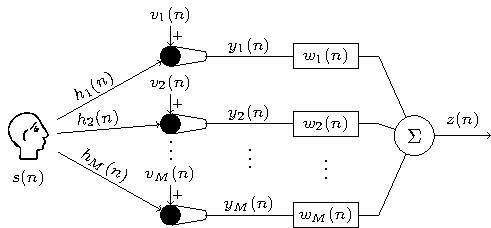
\includegraphics[scale=0.8]{Plots/configuration}
  \caption{Acoustic system configuration.}
  \label{fig: conf}
\end{figure}
The $m$th microphone signal $y_m(n)$, $m = 1, \ldots, M,$ at time index $n$ is given by 
\begin{equation}
\!\!\!\!\!y_m(n) \!\!=\!\! \underbrace{\sum_{l = 0}^{L_h-1}h_m(l)s(n-l)}_{x_m(n)} + \; v_m(n) = x_m(n) + v_m(n),\!\!\!
\end{equation}
where $h_m(l)$, $l = 0, \; \ldots, \; L_h-1$, are the coefficients of the time-invariant RIR between the speech source and the $m$th microphone, $s(n)$ is the clean speech signal, $x_m(n)$ is the reverberant speech component, and $v_m(n)$ is the additive noise component.
Since this paper aims to investigate the dereverberation performance of acoustic multichannel equalization techniques, in the following it is assumed that $v_m(n) = 0$, hence $y_m(n) = x_m(n)$.

Using the filter-and-sum structure in Fig.~\ref{fig: conf}, the output signal $z(n)$ is equal to the sum of the filtered microphone signals, i.e.,
\begin{equation}
\label{eq: out_sig}
z(n) = \sum_{m=1}^M \sum_{l = 0}^{L_w-1} w_m(l) x_m(n-l),
\end{equation}
where $w_m(l)$, $l = 0, \; \ldots, \; L_w-1$, are the coefficients of the $L_w$-taps long filter applied to the $m$th microphone signal.
In vector notation, the RIR $\mathbf{h}_m$ and the filter $\mathbf{w}_m$ can be described as
\begin{equation*}
\!\!\!\!\!\!\mathbf{h}_m = [h_m(0)  \ldots  h_m(L_h\!\!-\!\!1)]^T\!\!\!, \mathbf{w}_m  = [w_m(0) \ldots w_m(L_w\!\!-\!\!1)]^T\!\!\!.
\end{equation*}
Using the $M L_w$-dimensional stacked filter vector $\mathbf{w} = [\mathbf{w}^T_1  \ldots \mathbf{w}^T_M]^T$, the equalized impulse response~(EIR) vector $\mathbf{c}$ of length $L_c = L_h+L_w-1$, i.e., $\mathbf{c} = [c(0) \ldots c(L_c-1)]^T$, can be expressed as
\begin{equation}
\label{eq: eir_vec}
\mathbf{c} = \mathbf{H}\mathbf{w},
\end{equation}
where  $\mathbf{H}$ denotes the $L_c \times ML_w$-dimensional multichannel convolution matrix of the RIRs, i.e., $\mathbf{H}  = [\mathbf{H}_1 \ldots \mathbf{H}_M]$, and
\begin{equation}
\mathbf{H}_m \! = \! \begin{bmatrix}
    h_m(0) & 0 &  \ldots & 0 \\
    h_m(1) & h_m(0) & \ddots & \vdots \\
    \vdots & h_m(1) & \ddots & 0 \\
    h_m(L_h\!-\!1) & \vdots & \ddots & h_m(0) \\
    0 & h_m(L_h\!-\!1) & \ddots & h_m(1) \\
    \vdots & \ddots & \ddots & \vdots \\
    0 & \ldots & 0 & h_m(L_h\!-\!1)
   \end{bmatrix}.
 \end{equation}
Defining the $L_c$--dimensional clean speech vector $\mathbf{s}(n) = [s(n) \ldots s(n-L_c+1)]^T$ and the $L_w$--dimensional $m$th reverberant signal vector $\mathbf{x}_m(n) = [x_m(n) \ldots x_m(n-L_w+1)]^T$, with $\mathbf{x}_m(n) = \mathbf{H}_m^T \mathbf{s}(n)$, the output signal $z(n)$ can be expressed as
\begin{equation}
\label{eq: outsig_vec}
z(n) \!\!=\!\! \sum_{m=1}^M \mathbf{w}_m^T\mathbf{x}_m(n) \!\!=\!\! \sum_{m=1}^M \mathbf{w}_m^T\mathbf{H}^T_m\mathbf{s}(n) \!\!=\!\! \underbrace{\mathbf{w}^T\mathbf{H}^T}_{\mathbf{c}^T}\mathbf{s}(n).
\end{equation}
As indicated by~(\ref{eq: outsig_vec}), the dereverberation performance of the speech enhancement system fully depends on the EIR vector $\mathbf{c}$.
For conciseness, the time index $n$ will be omitted when possible in the remainder of this paper.

% The output signal in~(\ref{eq: outsig_vec}) can also be expressed as
% \begin{equation}
% \label{eq: outsig_vecalter}
% z(n) = \sum_{m=1}^M \mathbf{x}_m^T(n)\mathbf{w}_m = \mathbf{x}^T(n)\mathbf{w},
% \end{equation}
% with $\mathbf{x}(n) = [\mathbf{x}^T_1(n) \ldots \mathbf{x}^T_M(n)]^T$ the $ML_w$--dimensional stacked reverberant signal vector.
% Based on~(\ref{eq: outsig_vecalter}), the $L_z$--dimensional output signal vector $\mathbf{z}(n)$, i.e., $\mathbf{z}(n) = [z(n) \ldots z(n-L_z+1)]^T$, can be written as $\mathbf{z}(n) = \mathbf{X}(n)\mathbf{w}$, where $\mathbf{X}(n)$ denotes the $L_z \times ML_w$--dimensional multichannel convolution matrix of the reverberant signals, i.e.,  $ \mathbf{X}(n) = [\mathbf{X}_1(n) \ldots \mathbf{X}_M(n)]$, with $\mathbf{X}_m(n)$ the $L_z \times L_w$-dimensional convolution matrix of $\mathbf{x}_m(n)$.
% For conciseness, the time index $n$ will be omitted when possible in the remainder of this paper.


\subsection{Acoustic Multichannel Equalization}
\label{sec: ac_tech}
Acoustic multichannel equalization techniques assume that measurements or estimates of the RIRs are available. 
Such techniques aim at speech dereverberation by designing a reshaping filter $\mathbf{w}$ such that the (weighted) EIR in~(\ref{eq: eir_vec}) is equal to a (weighted) dereverberated target EIR.
Since the true RIRs are typically not available in practice, the reshaping filter is designed using the perturbed multichannel convolution matrix $\hat{\mathbf{H}}$ constructed from the available RIRs $\hat{\mathbf{h}}_m$.
This matrix is equal to $\hat{\mathbf{H}} = \mathbf{H} + \mathbf{E}$, where $\mathbf{E}$ represents the convolution matrix of the RIR perturbations arising due to, e.g., temperature fluctuations~\cite{Elko03roomimpulse}, source-microphone geometry mismatches~\cite{cole1997position,Radlovic_ITSA_2000}, RIR estimation errors from blind and supervised system identification methods~\cite{Haque_SPL_2008,Lin_ITASLP_2012}, or microphone transfer function mismatches.
It should be noted that microphone transfer function mismatches result in convolutive RIR perturbations instead of additive perturbations. However, the techniques discussed in the remainder of this paper are independent of the type of RIR perturbations present in the system, as long as a model is available to characterize these perturbations. 

In this paper, we will focus on the RMCLS~\cite{Lim_ITASLP_2014} and PMINT~\cite{Kodrasi_ITASLP_2013} techniques, which compute the filter $\mathbf{w}$ as the solution to
\begin{equation}
\label{eq: syseq}
\mathbf{W}\hat{\mathbf{H}}\mathbf{w} = \mathbf{W}\mathbf{c}_t,
\end{equation}
with $\mathbf{W}$ an $L_c \times L_c$--dimensional diagonal weighting matrix and $\mathbf{c}_t$ the $L_c$--dimensional target EIR.
The definition of the weighting matrix $\mathbf{W}$ and the target EIR $\mathbf{c}_t$ for the RMCLS and PMINT techniques is presented in Tables~\ref{tbl: weighting} and~\ref{tbl: target} respectively, where $\tau$ denotes a delay, $L_d$ denotes the length of the direct path and early reflections, $\mathbf{I}$ denotes the $L_c \times L_c$--dimensional identity matrix, and $p \in \{1, \; \ldots, \; M \}$, i.e., for the PMINT technique, the direct path and the early reflections of the target EIR are controlled by the first part of one of the available RIRs.
Without loss of generality, other desired EIRs could also be used instead, as long as they are perceptually close to the true RIRs.
\begin{table}[b!]  \small
\begin{center}
  \caption{Definition of the weighting matrix $\mathbf{W}$ in~(\ref{eq: syseq}) for the RMCLS and PMINT techniques.}
  \label{tbl: weighting}
  \begin{tabularx}{\linewidth}{Xr} \toprule Technique & Weighting
matrix $\mathbf{W}$ \\ \midrule RMCLS & $ { \mathrm{diag}} [
\underbrace {1 \; \ldots \; 1}_{\tau} \; \underbrace{1 \; 0 \; \ldots
\; 0}_{L_d} \; 1 \; \ldots 1]^{T} $\\ PMINT & $\mathbf{I}$ \\
\bottomrule
  \end{tabularx}
\end{center}
\end{table}
\begin{table}[b!]
\small
\begin{center}
  \caption{Definition of the target EIR $\mathbf{c}_t$ in~(\ref{eq: syseq}) for the \newline RMCLS and PMINT techniques.}
  \label{tbl: target}
  \begin{tabularx}{\linewidth}{Xr}
    \toprule
    Technique & Target EIR $\mathbf{c}_t$ \\
    \midrule
    RMCLS & $[\underbrace{0 \; \ldots \; 0}_{\tau} \; 1 \; 0 \; \ldots \; 0 ]^T$\\
    PMINT &  $[\underbrace{0\phantom{\rlap{$(L_d-1)$}} \ldots 0 }_{\tau} \underbrace{\hat{h}_p(0) \ldots \hat{h}_p(L_d-1)}_{L_d} 0 \ldots 0 ]^{T}$\\
    \bottomrule
  \end{tabularx}
\end{center}
\end{table}
From these definitions of $\mathbf{W}$ and $\mathbf{c}_t$, it can be observed that on the one hand, the RMCLS technique does not constrain all taps of the EIR, aiming only at suppressing the reverberant tail, while on the other hand, the PMINT technique constrains all taps of the EIR, aiming at suppressing the reverberant tail and preserving the perceptual speech quality.
For more details on these techniques, we refer to~\cite{Lim_ITASLP_2014,Kodrasi_ITASLP_2013}.

The filter solving~(\ref{eq: syseq}) is computed by minimizing the least-squares cost function\footnote{Strictly speaking, the cost function in~(\ref{eq: jls}) is a weighted least-squares cost function for $\mathbf{W} \neq \mathbf{I}$.} 
\begin{equation}
\label{eq: jls}
J_{_{\text{LS}}} = \|\mathbf{W} (\hat{\mathbf{H}}\mathbf{w} - \mathbf{c}_t) \|_2^2.
\end{equation} 
As shown in~\cite{Miyoshi_ITASS_1988,Kodrasi_ITASLP_2013}, assuming that the RIRs $\hat{\mathbf{h}}_m$ do not share any common zeros and using $L_w \geq \left\lceil{\frac{L_h-1}{M-1}}\right\rceil$, with $\left\lceil{\cdot}\right\rceil$ the ceiling operator, the filter minimizing~(\ref{eq: jls}) is equal to
\begin{equation}
\label{eq: w_ls}
\mathbf{w}_{_{\text{LS}}} = (\mathbf{W}\hat{\mathbf{H}})^+\mathbf{W}\mathbf{c}_t,
\end{equation}
where $\{ \cdot \}^+$ denotes the matrix pseudo-inverse. 
When the true RIRs are available, i.e., $\hat{\mathbf{H}} = \mathbf{H}$, this filter yields perfect dereverberation performance, i.e., $\mathbf{W}\mathbf{H}\mathbf{w}_{_{\text{LS}}} = \mathbf{W}\mathbf{c}_t$~\cite{Kodrasi_ITASLP_2013}.
However, in the presence of RIR perturbations, i.e., $\hat{\mathbf{H}} \neq \mathbf{H}$, this filter typically fails to achieve dereverberation, i.e., $\mathbf{W}\mathbf{H}\mathbf{w}_{_{\text{LS}}} \neq \mathbf{W}\mathbf{c}_t$, possibly even causing large distortions in the output signal~\cite{Kodrasi_ITASLP_2013}.

\subsection{Increasing Robustness Against RIR Perturbations}
\label{sec: robust_sec}
In this section, several methods that have been proposed to increase the robustness of the RMCLS and PMINT techniques are briefly reviewed.
Furthermore, insights on the computational complexity of these different methods are provided.
\vskip 2pt
\textbf{Decreasing the reshaping filter length:} \enspace
In~\cite{Kodrasi_EUSIPCO_2012} it was analytically shown that using a shorter reshaping filter length than conventionally used, i.e., $L_w < \left\lceil{\frac{L_h-1}{M-1}}\right\rceil$, decreases the condition number of the matrix $\mathbf{W}\hat{\mathbf{H}}$.
% , defined as
% \begin{equation}
% \kappa  = \frac{\sigma_{1}(\mathbf{W}\hat{\mathbf{H}})}{\sigma_{L}(\mathbf{W}\hat{\mathbf{H}})},
% \end{equation}
% where $\sigma_{1}(\mathbf{W}\hat{\mathbf{H}})$ and $\sigma_{L}(\mathbf{W}\hat{\mathbf{H}})$ denote the largest and smallest non-zero singular value of $\mathbf{W}\hat{\mathbf{H}}$.
As analytically shown in~\cite{Wedin_1973}, a smaller condition number yields a better-conditioned least-squares optimization criterion, with the resulting least-squares solution $\mathbf{w}_{_{\text{LS}}}$ in~(\ref{eq: w_ls}) being less sensitive to perturbations in $\mathbf{W}\hat{\mathbf{H}}$.
%Simulation results in~\cite{Kodrasi_EUSIPCO_2012} have shown that decreasing the reshaping filter length increases the robustness of the RMCLS and PMINT techniques against RIR perturbations.

\vskip 2pt
\textbf{Incorporating regularization:} \enspace
In~\cite{Kodrasi_ITASLP_2013} it was proposed to increase the robustness of the RMCLS and PMINT techniques by incorporating regularization in the filter design, such that the distortion energy due to RIR perturbations is reduced.
The regularized least-squares cost function is given by
\begin{equation}
\label{eq: jrls}
J_{_{\text{RLS}}} = \|\mathbf{W} (\hat{\mathbf{H}}\mathbf{w} - \mathbf{c}_t) \|_2^2 + \delta \mathbf{w}^T\mathbf{R}_{\mathbf{e}}\mathbf{w},
\end{equation}
with $\mathbf{R}_{\mathbf{e}}$ denoting the matrix modeling the perturbations, i.e., $\mathbf{R}_{\mathbf{e}} = {\cal{E}} \{\mathbf{E}^T\mathbf{E} \}$, where ${\cal{E}}$ denotes the expected value operator, and $\delta$ is a regularization parameter providing a trade-off between the minimization of the least-squares error $J_{_{\text{LS}}}$ and the distortion energy due to RIR perturbations $\mathbf{w}^T\mathbf{R}_{\mathbf{e}}\mathbf{w}$.
The regularized least-squares filter minimizing~(\ref{eq: jrls}) is given by
\begin{equation}
\label{eq: w_rls}
\mathbf{w}_{_{\text{RLS}}} = [ (\mathbf{W}\hat{\mathbf{H}})^T(\mathbf{W}\hat{\mathbf{H}})+\delta \mathbf{R}_{\mathbf{e}} ]^{-1}(\mathbf{W}\hat{\mathbf{H}})^T\mathbf{W}\mathbf{c}_t.
\end{equation}
%Simulation results in~\cite{Kodrasi_ITASLP_2013} have shown that incorporating regularization significantly increases the robustness of the RMCLS and PMINT techniques against RIR perturbations.
\vskip 2pt
\textbf{Incorporating sparsity-promoting penalty functions:} \enspace In~\cite{Kodrasi_ICASSP_2016,Kodrasi_ITASLP_2016b} it was proposed to increase the robustness of the RMCLS and PMINT techniques by incorporating penalty functions that promote sparsity of the output signal in the short-time Fourier transform (STFT) domain, such that the output signal exhibits characteristics of a clean speech signal.
The $L_z$-dimensional output signal vector $\mathbf{z} = [z(n) \; \ldots \; z(n-L_z+1)]^T$ can be expressed as
\begin{equation}
\mathbf{z} = \mathbf{X}\mathbf{w},
\end{equation}
where $\mathbf{X}$ denotes the $L_z \times ML_w$-dimensional multichannel convolution matrix of the microphone signals, i.e., $ \mathbf{X} = [\mathbf{X}_1 \; \mathbf{X}_2 \; \ldots \; \mathbf{X}_M]$, and
\begin{equation}
\mathbf{X}_m = \begin{bmatrix}
    x_m(n) &   \cdots & x_m(n-L_w+ 1) \\
    x_m(n-1) & \cdots & x_m(n-L_w) \\
    \vdots & \ddots & \vdots \\
    x_m(n-L_z+1) & \cdots & x_m(n-L_w-L_z+2)
   \end{bmatrix}\!\!\!.\!\!\!
 \end{equation}
The sparsity-promoting least-squares cost function is then given by
\begin{equation}
\label{eq: jsls}
J_{_{\text{SLS}}} = \|\mathbf{W} (\hat{\mathbf{H}}\mathbf{w} - \mathbf{c}_t) \|_2^2 + \eta f_{_{\text{SP}}} (\bm{\Psi}\mathbf{z} ),
\end{equation}
where $f_{_{\text{SP}}}$ denotes a sparsity-promoting penalty function and $\eta$ is a weighting parameter providing a trade-off between the minimization of the least-squares error $J_{_{\text{LS}}}$ and the penalty function value $f_{_{\text{SP}}}(\bm{\Psi}\mathbf{z})$.
The operator $\bm{\Psi}$ denotes the STFT operator transforming the $L_{z}$-dimensional time-domain vector $\mathbf{z}$ into the $L_{\tilde{z}}$-dimensional time-frequency domain vector $\tilde{\mathbf{z}}$ consisting of the STFT coefficients of the output signal, with $\tilde{\mathbf{z}} = \bm{\Psi}\mathbf{z}$.
Since no closed-form expression is available for the filter minimizing the cost function in~(\ref{eq: jsls}), the sparsity-promoting least-squares filter can be computed using, e.g., the iterative alternating direction method of multipliers~(ADMM) algorithm~\cite{Boyd_admm_2011}.
% Defining $\bm{\Psi} \in {\cal{C}}^{L_{\tilde{z}}\times L_z}$ as the STFT operator which transforms the $L_z$-dimensional time-domain output signal vector $\mathbf{z}$ into the $L_{\tilde{z}}$--dimensional time-frequency domain vector $\tilde{\mathbf{z}}$ consisting of the STFT coefficients of the output signal, i.e., $\tilde{\mathbf{z}} = \bm{\Psi}\mathbf{z}$, the sparsity-promoting least-squares cost function is given by
% \begin{align}
% J_{_{\text{SLS}}} & = \|\mathbf{W} (\hat{\mathbf{H}}\mathbf{w} - \mathbf{c}_t) \|_2^2 + \eta f_{_{\text{SP}}}(\tilde{\mathbf{z}}), \\
% \label{eq: jsls}
% & = \|\mathbf{W} (\hat{\mathbf{H}}\mathbf{w} - \mathbf{c}_t) \|_2^2 + \eta f_{_{\text{SP}}}(\bm{\Psi}\mathbf{X}\mathbf{w}),
% \end{align}
% where $f_{_{\text{SP}}}$ denotes a sparsity-promoting penalty function, e.g., $l_0$-norm, $l_1$-norm, or weighted $l_1$-norm, and $\eta$ is a weighting parameter providing a trade-off between the minimization of the least-squares error and the penalty function value.
% Since no closed-form expression is available for the filter minimizing the sparsity-promoting cost function in~(\ref{eq: jsls}), the sparsity-promoting least-squares filter is computed using the iterative alternating direction method of multipliers~(ADMM)~\cite{Boyd_admm_2011}.
% The ADMM algorithm minimizes 
% % \begin{equation}
% % \label{eq: lag}
% % \!\!\!\!\!\!\!\!\!\!{\cal{L}} \!\!=\!\! \|\mathbf{W}(\hat{\mathbf{H}}\mathbf{w}-\mathbf{c}_t) \|_2^2 \!\!+\!\! \eta f_{_{\text{SP}}}(\tilde{\mathbf{a}}) \!\!+\!\! \frac{\rho}{2} \|\bm{\Psi}\mathbf{X}\mathbf{w} +\bm{\lambda} - \tilde{\mathbf{a}}\|_2^2,\!\!\!\!
% % \end{equation}
% % with $\tilde{\mathbf{a}}$ an auxilary variable introduced such that the optimization problem in~(\ref{eq: jsls}) can be split into simpler sub-problems, $\bm{\lambda}$ the dual (splitting) variable, and $\rho>0$ the ADMM penalty parameter.
% % Within the ADMM framework, the minimization of the sparsity-promoting cost function in~(\ref{eq: jsls}) is reformulated as
% % \begin{equation}
% % \label{eq: cost_reform}
% % \!\!\!\!\!\!\!\min_{\mathbf{w}} \left[ \|\mathbf{W}(\hat{\mathbf{H}}\mathbf{w}-\mathbf{c}_t) \|_2^2 + \eta f_{_{\text{SP}}}(\tilde{\mathbf{a}}) \right] \; \; {\text{subject to}} \; \; \bm{\Psi}\mathbf{X}\mathbf{w} = \tilde{\mathbf{a}},
% % \end{equation}
% % where the auxiliary variable $\tilde{\mathbf{a}}$ is introduced such that the optimization problem in~(\ref{eq: jsls}) can be split into simpler sub-problems.
% % The augmented Lagrangian of~(\ref{eq: cost_reform}) is equal to
% % \begin{equation}
% % \label{eq: lag}
% % \!\!\!\!\!\!\!\!\!\!{\cal{L}} \!\!=\!\! \|\mathbf{W}(\hat{\mathbf{H}}\mathbf{w}-\mathbf{c}_t) \|_2^2 \!\!+\!\! \eta f_{_{\text{SP}}}(\tilde{\mathbf{a}}) \!\!+\!\! \frac{\rho}{2} \|\bm{\Psi}\mathbf{X}\mathbf{w} +\bm{\lambda} - \tilde{\mathbf{a}}\|_2^2,\!\!\!\!
% % \end{equation}
% % with $\bm{\lambda}$ the dual (splitting) variable and $\rho>0$ the ADMM penalty parameter.
Introducing the auxiliary variable $\mathbf{a}$ such that the optimization problem in~(\ref{eq: jsls}) is split into simpler sub-problems, the ADMM algorithm computes the sparsity-promoting least-squares filter using the following update rules~\cite{Kodrasi_ICASSP_2016,Kodrasi_ITASLP_2016b} until a termination criterion is satisfied~(cf. Section~\ref{sec: exp}):
{\footnotesize{
\begin{align}
\label{eq: w_admm_sls0}
\begin{split}
\mathbf{w}^{(i+1)} & = [ 2 (\mathbf{W}\hat{\mathbf{H}})^T(\mathbf{W}\hat{\mathbf{H}}) + \rho \mathbf{X}^T \mathbf{X} ]^{-1} \\
 &\quad \times [2 (\mathbf{W}\hat{\mathbf{H}})^T (\mathbf{W}\mathbf{c}_t) + \rho \mathbf{X}^T \bm{\Psi}^H \!({\mathbf{a}}^{(i)} - \bm{\lambda}^{(i)})],
\end{split} \\
\label{eq: aux_update}
{\mathbf{a}}^{(i+1)} & = S_{\eta / \rho}(\bm{\Psi}\mathbf{X}\mathbf{w}^{(i+1)} + \bm{\lambda}^{(i)}), \\
\label{eq: up_lambda_sls}
\bm{\lambda}^{(i+1)} & = \bm{\lambda}^{(i)} + \bm{\Psi}\mathbf{X}\mathbf{w}^{(i+1)} - {\mathbf{a}}^{(i+1)}.
\end{align}}}%
In~(\ref{eq: w_admm_sls0})-(\ref{eq: up_lambda_sls}), $\{\cdot\}^{(i)}$ denotes the variable in the $i$th iteration, $\bm{\lambda}$ is the so-called dual (splitting) variable, $\rho>0$ is the ADMM penalty parameter, and $S_{\eta/\rho}$ denotes the proximal mapping of the used sparsity-promoting penalty function~\cite{parikh2014proximal}.
Simulation results in~\cite{Kodrasi_ITASLP_2016b} have shown that incorporating an $l_0$-norm, $l_1$-norm, or weighted $l_1$-norm sparsity-promoting penalty function significantly increases the robustness of the RMCLS and PMINT techniques, with the weighted $l_1$-norm penalty function yielding the best performance.
Hence, in this paper we only consider the weighted $l_1$-norm penalty function, defined as
\begin{equation}
f_{_{\text{SP}}}(\tilde{\mathbf{z}}) = \|{\text{diag}}\{\mathbf{u} \}\tilde{\mathbf{z}}\|_1 = \sum_{q = 0}^{L_{\tilde{z}}-1} |u(q) \tilde{z}(q)|,
\end{equation}
with $u(q) > 0$, $q = 0, \ldots, L_{\tilde{z}}-1,$ denoting user-defined scalar weights.
In order to preserve the spectro-temporal structure of a typical speech signal, the weights $u(q)$ are defined as~\cite{Kodrasi_ITASLP_2016b}
\begin{equation}
\label{eq: weights}
u(q) = \frac{1}{|\tilde{x}_p(q)| + \zeta}, \; \; \; \; q = 0, \; \ldots, \; L_{\tilde{z}}-1,
\end{equation}
with $\tilde{x}_p(q)$ the STFT coefficients of the $p$-th microphone signal, where $p \in \{1, \; \ldots, \; M \}$, and $\zeta > 0$ a small positive scalar used to avoid division by $0$.
\vskip 2pt
While simulation results in~\cite{Kodrasi_EUSIPCO_2012, Kodrasi_ITASLP_2013,Kodrasi_ICASSP_2016, Kodrasi_ITASLP_2016b} have shown that all proposed methods are effective in increasing the robustness of the RMCLS and PMINT techniques against RIR perturbations, an extensive instrumental and perceptual comparison of the performance of all these methods to determine the most robust and perceptually advantageous technique is lacking.

\vskip 2pt
\textbf{Computational complexity considerations:} \enspace The computational complexity of all considered methods is at most cubic\footnote{This upper bound may be tightened when exploiting the fact that the matrices involved are symmetric or Toeplitz.}, since matrix multiplications and matrix inversions account for the dominant operations in all reshaping filter computations, cf.~(\ref{eq: w_ls}),~(\ref{eq: w_rls}), and~(\ref{eq: w_admm_sls0})-(\ref{eq: up_lambda_sls}).
The complexity of using a shorter reshaping filter length is $O(n_r^3)$, where $n_r$ denotes the number of rows of the matrix $\mathbf{W}\hat{\mathbf{H}}$ when $L_w < \left\lceil{\frac{L_h-1}{M-1}}\right\rceil$.
The complexity of using regularization is $O(n_c^3)$, where $n_c$ denotes the number of columns of the matrix $\mathbf{W}\hat{\mathbf{H}}$ when $L_w = \left\lceil{\frac{L_h-1}{M-1}}\right\rceil$.
Finally, the complexity of using a sparsity-promoting penalty function is $O(L_z^3)$, where $L_z$ denotes the length of the output signal vector. 
Since typically $n_r < n_c \ll L_z$, decreasing the reshaping filter length results in the lowest computational complexity, whereas incorporating a sparsity-promoting penalty function results in the highest computational complexity.
In addition, the execution of the sparsity-promoting method takes a significantly longer time than the execution of the other methods due to the multiple number of iterations. 

\section{ACOUSTIC SCENARIOS AND ALGORITHMIC SETTINGS}
\label{sec: exp}

This section describes the considered acoustic scenarios and the algorithmic settings for which the performance of the robust extensions of the RMCLS and PMINT techniques is evaluated.
% In addition, the intrumental measures used to evaluate the performance of the considered algorithms are introduced and a description of the subjective listening test setup is provided.

\textbf{Acoustic scenarios:} \enspace We considered $2$ different reverberant acoustic systems with a single speech source and $M = 4$ omni-directional microphones. 
For each acoustic system, Table~\ref{tbl: ac_sys} presents the reverberation time $T_{60}$, the source-microphone distance $d_{\text{sm}}$, the inter-microphone distance $d_{\text{im}}$, and the RIR length $L_h$ at a sampling frequency $f_s = 8$ kHz. 
The RIRs between the speech source and the microphones were measured using the swept-sine technique~\cite{Farina_2000} and the reverberant signals were generated by convolving $2$ sentences of clean speech (approximately $4$ s long) from the HINT database~\cite{Nilsson_JASA_1994} with the measured RIRs.
In order to simulate RIR perturbations, the measured RIRs were perturbed by proportional Gaussian distributed errors as proposed in~\cite{Zhang_HINDAWI_2008}, such that a desired normalized projection misalignment (NPM), defined as
\begin{equation}
{\text{NPM}} = 10 \log_{10} \frac{\left\| \mathbf{h}_m - \frac{\mathbf{h}_m^T\hat{\mathbf{h}}_m}{\hat{\mathbf{h}}_m^T\hat{\mathbf{h}}_m}\hat{\mathbf{h}}_m\right\|_2^2}{\| \mathbf{h}_m \|_2^2},
\end{equation}
is obtained. 
The considered NPMs are NPM$_1 = -33$ dB and NPM$_2 = -15$ dB, with NPM$_1$ representing a moderate perturbation level and NPM$_2$ representing a high perturbation level.
Hence, the performance of all considered techniques is evaluated for $4$ different acoustic scenarios, i.e., S$_1$-NPM$_1$, S$_2$-NPM$_1$, S$_1$-NPM$_2$, and S$_2$-NPM$_2$.

\begin{table}[b!]
\small
\begin{center}
  \caption{Characteristics of the considered acoustic systems.}
  \label{tbl: ac_sys}
  \begin{tabularx}{\linewidth}{Xrrrr}
    \toprule
    System & $T_{60}$ [ms] & $d_{\text{sm}}$ [m] & $d_{\text{im}}$ [m] & $L_h$  \\
    \midrule
    $\text{S}_1$ & $450$ & $3$ & $0.05$ & $3600$ \\
    $\text{S}_2$ & $610$ & $2$ & $0.04$ & $4880$ \\
    \bottomrule
  \end{tabularx}
\end{center}
\end{table}
\textbf{Algorithmic settings:} \enspace
As previously mentioned, we investigate the performance of the following techniques (cf. Section~\ref{sec: ac_tech}):
\begin{itemize}
  \item L-RMCLS, i.e., the RMCLS technique using a shorter reshaping filter length,
  \item R-RMCLS, i.e., the regularized RMCLS technique,
  \item S-RMCLS, i.e., the weighted $l_1$-norm sparsity-promoting RMCLS technique,
  \item L-PMINT, i.e., the PMINT technique using a shorter reshaping filter length,
  \item R-PMINT, i.e., the regularized PMINT technique, and
  \item S-PMINT, i.e., the weighted $l_1$-norm sparsity-promoting PMINT technique. 
\end{itemize}
For the R-RMCLS, S-RMCLS, R-PMINT, and S-PMINT techniques the reshaping filter length is set to $L_w = \left\lceil{\frac{L_h-1}{M-1}}\right\rceil$, i.e., $L_w = 1200$ for the system $S_1$ and $L_w = 1627$ for the system $S_2$. 
As shown in~\cite{Miyoshi_ITASS_1988}, this filter length is the minimum length required for perfect dereverberation performance.
For all techniques, the delay is set to $\tau = 90$ and the length of the direct path and early reflections is set to $L_d = 0.01 \times f_s$ (i.e., $10$ ms), cf. Tables~\ref{tbl: weighting} and~\ref{tbl: target}.
The target EIR $\mathbf{c}_t$ for the robust extensions of the PMINT technique is set to the direct path and early reflections of the first RIR $\hat{\mathbf{h}}_1$, i.e., $p = 1$.
For the regularized techniques, the matrix $\mathbf{R}_{\mathbf{e}}$ modeling the RIR perturbations is set to $\mathbf{R}_{\mathbf{e}} = \mathbf{I}$.
For the sparsity-promoting techniques, the STFT is computed using a $32$ ms Hamming window with $50 \%$ overlap between successive frames. 
As in~\cite{Kodrasi_ICASSP_2016}, the variables $\mathbf{w}$, ${\mathbf{a}}$, and $\bm{\lambda}$ are initialized with $[1 \; 0 \ldots 0]^T$ and the termination criterion is set to either the number of iterations exceeding $150$ or the change in the filter norm dropping below $10^{-3}$.
The weights in~(\ref{eq: weights}) are computed using the STFT coefficients of the first microphone signal $\tilde{x}_1(q)$, i.e., $p = 1$.

The considered reshaping filter lengths $L_w$ for the L-RMCLS and L-PMINT techniques, regularization parameters $\delta$ for the R-RMCLS and R-PMINT techniques, and weighting and penalty parameters $\eta$ and $\rho$ for the S-RMCLS and S-PMINT techniques are
\begin{align}
\label{eq: pars}
L_w & \in \{ 500, 600, \ldots, \left\lceil{\frac{L_h-1}{M-1}}\right\rceil \}, \\
\delta & \in \{10^{-7}, 10^{-6}, \ldots, 10^{-1}, 1, 3, 5, 7, 10 \}, \\
\eta & \in \{ 10^{-7}, 10^{-6}, 10^{-5}, 10^{-4}\}, \\
\label{eq: par_last}
\rho & \in \{ 10^{-7}, 10^{-6}, \ldots, 10^{-1} \}.
\end{align}
As in~\cite{Kodrasi_EUSIPCO_2012, Kodrasi_ITASLP_2013}, the optimal reshaping filter length, the optimal regularization parameter, and the optimal weighting and penalty parameters used in the following simulations are intrusively selected from~(\ref{eq: pars})-(\ref{eq: par_last}) as the parameters maximizing the perceptual evaluation of speech quality (PESQ) score~\cite{PESQ} for each technique and each acoustic scenario (cf. Section~\ref{sec: obj} for details on the PESQ score computation). 
It should be noted that the computation of the PESQ score for selecting the optimal parameters is an intrusive procedure that is not applicable in practice, since knowledge of the true RIRs is required in order to compute the reference signal and the resulting EIR.


\section{INSTRUMENTAL EVALUATION}
\label{sec: obj}
In this section, the performance of the different considered techniques is evaluated by means of commonly used instrumental performance measures, i.e., direct-to-reverberant ratio (DRR)~\cite{Naylor_Derev_book}, speech-to-reverberation modulation energy ratio~(SRMR)~\cite{Santos_IWAENC_2014}, log likelihood ratio~(LLR)~\cite{Hu_ITASLP_2008}, and PESQ~\cite{PESQ}.
The channel-based DRR measure has been shown to correlate well with the perceived amount of reverberation for unprocessed signals~\cite{Cauchi_ICASSP_2016}, whereas the signal-based SRMR, LLR, and PESQ measures have been shown to correlate well with the perceived overall quality of signals processed by speech enhancement algorithms for dereverberation and noise reduction~\cite{Kinoshita_EURASIP_2016}.
While the SRMR measure is a non-intrusive measure, the LLR and PESQ measures are intrusive measures comparing the output signal to a (dereverberated) reference signal.
The reference signal employed in this evaluation is the clean speech signal convolved with the direct path and the early reflections (up to $10$ ms) of the true RIR $\mathbf{h}_1$.
Note that a higher DRR, a higher SRMR, a lower LLR, and a higher PESQ score indicate a better performance.

Fig.~\ref{fig: objective}a depicts the obtained DRR for the input RIR $\mathbf{h}_1$ and for the EIRs $\mathbf{c}$ obtained using the robust extensions of the RMCLS and PMINT techniques.
%, SRMR, LLR, and PESQ score for the reverberant microphone signal $x_1(n)$ and for the output signals $z(n)$ obtained using the robust extensions of the RMCLS and PMINT techniques.
\begin{figure*}[t!]
\centering
\begin{tikzpicture}[font = \small]

\begin{axis}[%
width=0.95\figurewidth,
height=0.5\figureheight,
area legend,
scale only axis,
xmin=0.5,
xmax=4.5,
xticklabels = {\empty},
xtick={1, 2, 3, 4},
xmajorgrids,
ymin=-2,
ymax=18,
ylabel={DRR [dB]},
xlabel absolute, xlabel style={yshift=1em},
ylabel absolute, ylabel style={yshift=-1.0em},
ymajorgrids,
 legend style={at={(.5,1.07)},anchor=south},
    legend cell align=left,
    legend columns=7,
]
\addplot[ybar,bar width=0.0228571428571429\figurewidth,bar shift=-0.0857142857142857\figurewidth,pattern = crosshatch,draw=black] plot coordinates{(1,0.246741536823367)
(2,-1.88720309257993)
(3,0.246741536823367)
(4,-1.88720309257993)};

\addlegendentry{$\mathbf{h}_1$, $x_1(n)$};

\addplot [
color=black,
solid,
forget plot
]
table[row sep=crcr]{
0.5 0\\
4.5 0\\
};
\addplot[ybar,bar width=0.0228571428571429\figurewidth,bar shift=-0.0571428571428571\figurewidth,fill=black!30!white,draw=black] plot coordinates{(1,16.1478432907784)
(2,5.20260927352776)
(3,6.11750456797714)
(4,1.66714103297406)};

\addlegendentry{L-RMCLS};

\addplot[ybar,bar width=0.0228571428571429\figurewidth,bar shift=-0.0285714285714286\figurewidth,pattern = north east lines,draw=black] plot coordinates{(1,16.6898602165705)
(2,9.281000253096)
(3,12.5763387156477)
(4,8.94615058689066)};

\addlegendentry{R-RMCLS};

\addplot[ybar,bar width=0.0228571428571429\figurewidth,fill=white,draw=black] plot coordinates{(1,14.3981689684257)
(2,14.5502490504388)
(3,8.49992681392159)
(4,6.3147594504873)};

\addlegendentry{S-RMCLS};

\addplot[ybar,bar width=0.0228571428571429\figurewidth,bar shift=0.0285714285714286\figurewidth,pattern = dots,draw=black] plot coordinates{(1,9.53524246437137)
(2,5.18643718083089)
(3,4.80599794901243)
(4,2.06800681471206)};

\addlegendentry{L-PMINT};

\addplot[ybar,bar width=0.0228571428571429\figurewidth,bar shift=0.0571428571428572\figurewidth,fill=black!50!white,draw=black] plot coordinates{(1,10.9312320796817)
(2,10.5190625620341)
(3,9.67170383008862)
(4,7.47051017107904)};

\addlegendentry{R-PMINT};

\addplot[ybar,bar width=0.0228571428571429\figurewidth,bar shift=0.0857142857142857\figurewidth,pattern = north west lines,draw=black] plot coordinates{(1,10.8208547812845)
(2,9.48121961068157)
(3,8.56635393136103)
(4,4.97993618364822)};

\addlegendentry{S-PMINT};

\end{axis}
\node[left, yshift = -8pt] at (current bounding box.west) {(a)};
\end{tikzpicture}%

\begin{tikzpicture}[font = \small]

\begin{axis}[%
width=0.95\figurewidth,
height=0.5\figureheight,
area legend,
scale only axis,
xmin=0.5,
xmax=4.5,
xtick={1, 2, 3, 4},
xmajorgrids,
xticklabels = {\empty},
ymin=0,
xlabel absolute, xlabel style={yshift=1em},
ylabel absolute, ylabel style={yshift=-1.0em},
ymax=5,
ylabel={SRMR [dB]},
ymajorgrids
]
\addplot[ybar,bar width=0.0228571428571429\figurewidth,bar shift=-0.0857142857142857\figurewidth,pattern = crosshatch,draw=black] plot coordinates{(1,2.86229416723948)
(2,3.38134297503546)
(3,2.40672165081228)
(4,2.57853195529855)};

\addplot [
color=black,
solid,
forget plot
]
table[row sep=crcr]{
0.5 0\\
4.5 0\\
};
\addplot[ybar,bar width=0.0228571428571429\figurewidth,bar shift=-0.0571428571428571\figurewidth,fill=black!30!white,draw=black] plot coordinates{(1,3.12202111918601)
(2,2.04642636619851)
(3,2.46158733891924)
(4,1.57973654032265)};

\addplot[ybar,bar width=0.0228571428571429\figurewidth,bar shift=-0.0285714285714286\figurewidth,pattern = north east lines,draw=black] plot coordinates{(1,3.70471078657045)
(2,3.71830201801369)
(3,3.34771900809086)
(4,2.88880826298988)};

\addplot[ybar,bar width=0.0228571428571429\figurewidth,fill=white,draw=black] plot coordinates{(1,4.05873506755622)
(2,3.83600472550323)
(3,3.21790539212663)
(4,3.04280530449869)};

\addplot[ybar,bar width=0.0228571428571429\figurewidth,bar shift=0.0285714285714286\figurewidth,pattern = dots,draw=black] plot coordinates{(1,3.30596628836935)
(2,3.60454420878151)
(3,2.30863725472184)
(4,2.11758975384415)};

\addplot[ybar,bar width=0.0228571428571429\figurewidth,bar shift=0.0571428571428572\figurewidth,fill=black!50!white,draw=black] plot coordinates{(1,4.11791141570958)
(2,4.509545009426)
(3,3.26881009947187)
(4,2.51166015734681)};

\addplot[ybar,bar width=0.0228571428571429\figurewidth,bar shift=0.0857142857142857\figurewidth,pattern = north west lines,draw=black] plot coordinates{(1,4.0276207278747)
(2,4.34938655397359)
(3,3.46604980971217)
(4,2.61310443743498)};

\end{axis}
\node[left, yshift = 0pt] at (current bounding box.west) {(b)};
\end{tikzpicture}%

\begin{tikzpicture}[font = \small]

\begin{axis}[%
width=0.95\figurewidth,
height=0.5\figureheight,
area legend,
scale only axis,
xmin=0.5,
xmax=4.5,
xtick={1, 2, 3, 4},
xlabel absolute, xlabel style={yshift=1em},
xticklabels = {\empty},
xmajorgrids,
ymin=0,
ymax=1.4,
ylabel={LLR [dB]},
ylabel absolute, ylabel style={yshift=-1.0em},
ymajorgrids
]
\addplot[ybar,bar width=0.0228571428571429\figurewidth,bar shift=-0.0857142857142857\figurewidth,pattern = crosshatch,draw=black] plot coordinates{(1,0.617661937930832)
(2,0.63336032545432)
(3,0.610987649834872)
(4,0.653771637993151)};

\addplot [
color=black,
solid,
forget plot
]
table[row sep=crcr]{
0.5 0\\
4.5 0\\
};
\addplot[ybar,bar width=0.0228571428571429\figurewidth,bar shift=-0.0571428571428571\figurewidth,fill=black!30!white,draw=black] plot coordinates{(1,0.953979370087267)
(2,1.37056437843726)
(3,0.702583232740106)
(4,1.14551809282901)};

\addplot[ybar,bar width=0.0228571428571429\figurewidth,bar shift=-0.0285714285714286\figurewidth,pattern = north east lines,draw=black] plot coordinates{(1,0.438965692377659)
(2,0.996969423781351)
(3,0.580605300537768)
(4,0.770469426233141)};

\addplot[ybar,bar width=0.0228571428571429\figurewidth,fill=white,draw=black] plot coordinates{(1,0.416345525084223)
(2,1.0366356826971)
(3,0.661262775370622)
(4,0.961231371414626)};

\addplot[ybar,bar width=0.0228571428571429\figurewidth,bar shift=0.0285714285714286\figurewidth,pattern = dots,draw=black] plot coordinates{(1,0.427022247219018)
(2,0.66862168399789)
(3,0.73517292043884)
(4,0.760761269674389)};

\addplot[ybar,bar width=0.0228571428571429\figurewidth,bar shift=0.0571428571428572\figurewidth,fill=black!50!white,draw=black] plot coordinates{(1,0.290772006919252)
(2,0.376702432937691)
(3,0.469472480987735)
(4,0.622086775790926)};

\addplot[ybar,bar width=0.0228571428571429\figurewidth,bar shift=0.0857142857142857\figurewidth,pattern = north west lines,draw=black] plot coordinates{(1,0.337368220144609)
(2,0.489246700284736)
(3,0.654379591494599)
(4,0.846185280452319)};

\end{axis}
\node[left, yshift = 3pt] at (current bounding box.west) {(c)};
\end{tikzpicture}%

\begin{tikzpicture}[font = \small]

\begin{axis}[%
width=0.95\figurewidth,
height=0.5\figureheight,
area legend,
scale only axis,
xmin=0.5,
xmax=4.5,
xtick={1, 2, 3, 4},
xticklabels={S$_1$-NPM$_1$, S$_2$-NPM$_1$, S$_1$-NPM$_2$, S$_2$-NPM$_2$},
xlabel = {Scenario},
xmajorgrids,
ymin=0,
ymax=4,
ylabel={PESQ},
xlabel absolute, xlabel style={align = center, yshift=0.2em},
ylabel absolute, ylabel style={yshift=-1.0em},
ymajorgrids
]
\addplot[ybar,bar width=0.0228571428571429\figurewidth,bar shift=-0.0857142857142857\figurewidth,pattern = crosshatch,draw=black] plot coordinates{(1,1.695)
(2,1.615)
(3,1.741)
(4,1.736)};

\addplot [
color=black,
solid,
forget plot
]
table[row sep=crcr]{
0.5 0\\
4.5 0\\
};
\addplot[ybar,bar width=0.0228571428571429\figurewidth,bar shift=-0.0571428571428571\figurewidth,fill=black!30!white,draw=black] plot coordinates{(1,2.644)
(2,2.148)
(3,1.922)
(4,1.749)};

\addplot[ybar,bar width=0.0228571428571429\figurewidth,bar shift=-0.0285714285714286\figurewidth,pattern = north east lines,draw=black] plot coordinates{(1,3.748)
(2,3.53)
(3,2.758)
(4,2.256)};

\addplot[ybar,bar width=0.0228571428571429\figurewidth,fill=white,draw=black] plot coordinates{(1,3.039)
(2,3.025)
(3,2.339)
(4,2.154)};

\addplot[ybar,bar width=0.0228571428571429\figurewidth,bar shift=0.0285714285714286\figurewidth,pattern = dots,draw=black] plot coordinates{(1,2.421)
(2,1.896)
(3,1.927)
(4,1.836)};

\addplot[ybar,bar width=0.0228571428571429\figurewidth,bar shift=0.0571428571428572\figurewidth,fill=black!50!white,draw=black] plot coordinates{(1,3.534)
(2,3.224)
(3,2.692)
(4,2.273)};

\addplot[ybar,bar width=0.0228571428571429\figurewidth,bar shift=0.0857142857142857\figurewidth,pattern = north west lines,draw=black] plot coordinates{(1,3.428)
(2,2.906)
(3,2.612)
(4,2.178)};

\end{axis}
\node[left, yshift = 10pt] at (current bounding box.west) {(d)};
\end{tikzpicture}%
\vspace{-0.3cm}
  \caption{Instrumental measures for the robust extensions of the RMCLS and PMINT techniques for all considered acoustic scenarios: (a) DRR, (b) SRMR, (c) LLR, and (d) PESQ.}
  \label{fig: objective}
\end{figure*}
The following conclusions can be drawn by comparing the presented DRR values:
\begin{itemize}
\item All techniques improve the DRR in comparison to the input RIR $\mathbf{h}_1$.
\item The robust extensions of the RMCLS technique generally yield a similar or higher DRR than the robust extensions of the PMINT technique.
This is to be expected since the robust extensions of the RMCLS technique relax the constraints on the filter design and aim only at suppressing the late reverberation, whereas the robust extensions of the PMINT technique also aim at preserving the perceptual speech quality (which is not reflected by the DRR measure).
\item The R-RMCLS technique typically yields the highest DRR for the considered scenarios (except for the scenario S$_2$-NPM$_1$, where the S-RMCLS technique yields the highest DRR).
\item The R-PMINT technique typically yields a higher DRR than the S-PMINT technique (except for the scenario S$_1$-NPM$_1$, where the R-PMINT and S-PMINT techniques yield a similar DRR).
\item The L-RMCLS and L-PMINT techniques yield the lowest DRR out of all considered robust extensions. 
This is not surprising since these techniques simply use a shorter reshaping filter length, without explicitly taking into account the structure of the RIR perturbations or the characteristics of the output speech signal.
\item The performance of all considered techniques is generally higher for the system S$_1$ than for the system S$_2$. 
This can be explained by the higher reverberation time of the system S$_2$, leading to a larger number of perturbed RIR taps to be reshaped, and hence, an increased sensitivity of all considered techniques to RIR perturbations.
\end{itemize} 
Figs.~\ref{fig: objective}b-\ref{fig: objective}d depict the obtained SRMR, LLR, and PESQ scores for the reverberant microphone signal $x_1(n)$ and for the output signals $z(n)$ obtained using the robust extensions of the RMCLS and PMINT techniques.
The following conclusions can be drawn by comparing the presented instrumental measures:
\begin{itemize}
\item Not all techniques improve the overall quality in comparison to the reverberant signal $x_1(n)$, e.g., the L-RMCLS technique yields a lower SRMR for scenarios S$_2$-NPM$_1$ and S$_2$-NPM$_2$, the L-PMINT technique yields a lower SRMR for the scenario S$_2$-NPM$_2$, and the R-PMINT technique is the only technique consistently improving the LLR for all scenarios.
\item The robust extensions of the PMINT technique generally yield a similar or better SRMR and LLR than the robust extensions of the RMCLS technique. 
Surprisingly, the robust extensions of the RMCLS technique generally yield a similar or better PESQ score than the robust extensions of the PMINT technique, implying that PESQ does not appear to reflect the better preservation of the early reflections achieved by the robust extensions of the PMINT technique but puts more emphasis instead on the better reverberant tail suppression achieved by the robust extensions of the RMCLS technique.
\item The R-PMINT technique typically yields the best SRMR and LLR (except for the scenario S$_2$-NPM$_2$, where the S-RMCLS technique yields the best SRMR), whereas the R-RMCLS technique typically yields the best PESQ score. 
\item As expected, the L-RMCLS and L-PMINT techniques typically yield the lowest performance in terms of all instrumental performance measures.
\item The performance of all considered techniques is generally higher for the system S$_1$ than for the system S$_2$. 
\end{itemize}
In summary, based on instrumental performance measures it can be said that incorporating regularization and sparsity-promoting penalty functions is more advantageous to increase the robustness of equalization techniques than using a shorter reshaping filter length.
Furthermore, as expected, the robust extensions of the RMCLS technique achieve a larger reverberant energy suppression (as evaluated using the DRR measure) than the robust extensions of the PMINT technique, with the R-RMCLS technique typically yielding the best performance.
However, when comparing the perceptual speech quality achieved by the different techniques, different conclusions can be derived depending on the used instrumental performance measure, highlighting the necessity of conducting subjective listening tests.


\section{PERCEPTUAL RESULTS}
\label{sec: mushra}
The perceptual evaluation is based on a multi stimulus test with hidden reference and anchor (MUSHRA) using the specifications given in~\cite{MUSHRA}.
The evaluation is conducted for the reverberant microphone signal $x_1(n)$ and for the output signals $z(n)$ obtained using all considered techniques.
In addition to these signals, a hidden reference and an anchor are presented to the subjects. 
The hidden reference has been generated as the clean speech signal convolved with the direct path and the early reflections (up to $10$ ms) of the true RIR $\mathbf{h}_1$.
The anchor has been generated as the low-pass filtered microphone signal $x_1(n)$  with a cut-off frequency of $3$ kHz.
Sound samples for each considered acoustic scenario can be found at \url{bit.ly/mushrasamples}.
The signals are diotically presented to the subjects through headphones (Sennheiser HDA 200) using an RME Fireface UFX sound card, with all signals normalized in amplitude.
A total of $21$ self-reported normal hearing subjects who are familiar with speech processing participated in the listening tests.
The subjects evaluated the signals in terms of the attribute ``overall speech quality'' on a scale from $0$ to $100$. 
Prior to the actual evaluation, the subjects were trained to familiarize themselves with the task and the signals under test.
Furthermore, they could adjust the sound volume to a comfortable level.
The order of presentation of signals and scenarios were randomized between all subjects.

Fig.~\ref{fig: mushra} depicts the obtained MUSHRA scores for the reverberant microphone signal and for the output signals obtained using the robust extensions of the RMCLS and PMINT techniques.
For completeness, the obtained MUSHRA scores for the reference and the anchor are also depicted, illustrating that the reference is correctly identified for all scenarios and that the anchor is typically rated as having the worst perceptual speech quality (except for the scenario S$_2$-NPM$_1$, where the L-RMCLS technique yields a worse quality).
In general it can be observed that the rating variability between subjects~(as shown by the whiskers in each boxplot) is rather large. 
This is commonly the case for listening tests evaluating the overall speech quality achieved by dereverberation algorithms, e.g.,~\cite{Cauchi_EURASIP_2015,Warzybok_IWAENC_2014,Goetze_JAES_2014}.
Since the artifacts and distortions produced by the considered techniques are quite different, the perception of these artifacts and distortions by different subjects is also rather different.

\begin{figure*}[t!]
  \centering
\begin{tikzpicture}[font = \small]

\begin{axis}[%
width=\figurewidth,
height=\figureheight,
clip=false,
scale only axis,
xmin=0,
xmax=50,
area legend,
xtick={5,18,31,44},
xticklabels={S$_1$-NPM$_1$, S$_2$-NPM$_1$, S$_1$-NPM$_2$, S$_2$-NPM$_2$},
xlabel absolute, xlabel style={yshift=0.2em},
xlabel={Scenario},
xmajorgrids,
ymin=-5,
ymax=105,
ylabel={Score},
ytick = {0,20,40,60,80,100},
ylabel absolute, ylabel style={yshift=-1.0em},
ymajorgrids,
 legend style={at={(.5,1.07)},anchor=south, inner sep = 0pt,font = \footnotesize},
    legend cell align=left,
    legend columns=9,
]
\addplot [
color=black,
dashed,
forget plot
]
table[row sep=crcr]{
1 100\\
1 100\\
};
\addplot [
color=black,
dashed,
forget plot
]
table[row sep=crcr]{
2 15\\
2 22\\
};
\addplot [
color=black,
dashed,
forget plot
]
table[row sep=crcr]{
3 37\\
3 72\\
};
\addplot [
color=black,
dashed,
forget plot
]
table[row sep=crcr]{
4 34.75\\
4 49\\
};
\addplot [
color=black,
dashed,
forget plot
]
table[row sep=crcr]{
5 61.5\\
5 90\\
};
\addplot [
color=black,
dashed,
forget plot
]
table[row sep=crcr]{
6 72\\
6 98\\
};
\addplot [
color=black,
dashed,
forget plot
]
table[row sep=crcr]{
7 49.25\\
7 60\\
};
\addplot [
color=black,
dashed,
forget plot
]
table[row sep=crcr]{
8 84.5\\
8 96\\
};
\addplot [
color=black,
dashed,
forget plot
]
table[row sep=crcr]{
9 90\\
9 100\\
};
\addplot [
color=black,
dashed,
forget plot
]
table[row sep=crcr]{
14 100\\
14 100\\
};
\addplot [
color=black,
dashed,
forget plot
]
table[row sep=crcr]{
15 20.75\\
15 46\\
};
\addplot [
color=black,
dashed,
forget plot
]
table[row sep=crcr]{
16 37.75\\
16 58\\
};
\addplot [
color=black,
dashed,
forget plot
]
table[row sep=crcr]{
17 11.25\\
17 16\\
};
\addplot [
color=black,
dashed,
forget plot
]
table[row sep=crcr]{
18 57.75\\
18 72\\
};
\addplot [
color=black,
dashed,
forget plot
]
table[row sep=crcr]{
19 67.5\\
19 81\\
};
\addplot [
color=black,
dashed,
forget plot
]
table[row sep=crcr]{
20 37\\
20 63\\
};
\addplot [
color=black,
dashed,
forget plot
]
table[row sep=crcr]{
21 83.25\\
21 96\\
};
\addplot [
color=black,
dashed,
forget plot
]
table[row sep=crcr]{
22 77.75\\
22 92\\
};
\addplot [
color=black,
dashed,
forget plot
]
table[row sep=crcr]{
27 100\\
27 100\\
};
\addplot [
color=black,
dashed,
forget plot
]
table[row sep=crcr]{
28 12.75\\
28 17\\
};
\addplot [
color=black,
dashed,
forget plot
]
table[row sep=crcr]{
29 44\\
29 81\\
};
\addplot [
color=black,
dashed,
forget plot
]
table[row sep=crcr]{
30 52.5\\
30 80\\
};
\addplot [
color=black,
dashed,
forget plot
]
table[row sep=crcr]{
31 80\\
31 95\\
};
\addplot [
color=black,
dashed,
forget plot
]
table[row sep=crcr]{
32 58.25\\
32 97\\
};
\addplot [
color=black,
dashed,
forget plot
]
table[row sep=crcr]{
33 50\\
33 73\\
};
\addplot [
color=black,
dashed,
forget plot
]
table[row sep=crcr]{
34 78\\
34 97\\
};
\addplot [
color=black,
dashed,
forget plot
]
table[row sep=crcr]{
35 60.25\\
35 94\\
};
\addplot [
color=black,
dashed,
forget plot
]
table[row sep=crcr]{
40 100\\
40 100\\
};
\addplot [
color=black,
dashed,
forget plot
]
table[row sep=crcr]{
41 24.75\\
41 37\\
};
\addplot [
color=black,
dashed,
forget plot
]
table[row sep=crcr]{
42 45\\
42 63\\
};
\addplot [
color=black,
dashed,
forget plot
]
table[row sep=crcr]{
43 17.5\\
43 35\\
};
\addplot [
color=black,
dashed,
forget plot
]
table[row sep=crcr]{
44 65\\
44 81\\
};
\addplot [
color=black,
dashed,
forget plot
]
table[row sep=crcr]{
45 51.25\\
45 74\\
};
\addplot [
color=black,
dashed,
forget plot
]
table[row sep=crcr]{
46 61.75\\
46 70\\
};
\addplot [
color=black,
dashed,
forget plot
]
table[row sep=crcr]{
47 67.75\\
47 90\\
};
\addplot [
color=black,
dashed,
forget plot
]
table[row sep=crcr]{
48 53.75\\
48 78\\
};
\addplot [
color=black,
dashed,
forget plot
]
table[row sep=crcr]{
1 100\\
1 100\\
};
\addplot [
color=black,
dashed,
forget plot
]
table[row sep=crcr]{
2 0\\
2 3\\
};
\addplot [
color=black,
dashed,
forget plot
]
table[row sep=crcr]{
3 3\\
3 10.75\\
};
\addplot [
color=black,
dashed,
forget plot
]
table[row sep=crcr]{
4 0\\
4 9.5\\
};
\addplot [
color=black,
dashed,
forget plot
]
table[row sep=crcr]{
5 10\\
5 39.5\\
};
\addplot [
color=black,
dashed,
forget plot
]
table[row sep=crcr]{
6 21\\
6 51.25\\
};
\addplot [
color=black,
dashed,
forget plot
]
table[row sep=crcr]{
7 3\\
7 29.75\\
};
\addplot [
color=black,
dashed,
forget plot
]
table[row sep=crcr]{
8 40\\
8 50.75\\
};
\addplot [
color=black,
dashed,
forget plot
]
table[row sep=crcr]{
9 64\\
9 74\\
};
\addplot [
color=black,
dashed,
forget plot
]
table[row sep=crcr]{
14 100\\
14 100\\
};
\addplot [
color=black,
dashed,
forget plot
]
table[row sep=crcr]{
15 0\\
15 2.5\\
};
\addplot [
color=black,
dashed,
forget plot
]
table[row sep=crcr]{
16 0\\
16 13\\
};
\addplot [
color=black,
dashed,
forget plot
]
table[row sep=crcr]{
17 0\\
17 0\\
};
\addplot [
color=black,
dashed,
forget plot
]
table[row sep=crcr]{
18 6\\
18 29.25\\
};
\addplot [
color=black,
dashed,
forget plot
]
table[row sep=crcr]{
19 2\\
19 34.75\\
};
\addplot [
color=black,
dashed,
forget plot
]
table[row sep=crcr]{
20 3\\
20 19.25\\
};
\addplot [
color=black,
dashed,
forget plot
]
table[row sep=crcr]{
21 48\\
21 60\\
};
\addplot [
color=black,
dashed,
forget plot
]
table[row sep=crcr]{
22 27\\
22 54.75\\
};
\addplot [
color=black,
dashed,
forget plot
]
table[row sep=crcr]{
27 100\\
27 100\\
};
\addplot [
color=black,
dashed,
forget plot
]
table[row sep=crcr]{
28 0\\
28 1\\
};
\addplot [
color=black,
dashed,
forget plot
]
table[row sep=crcr]{
29 0\\
29 14.75\\
};
\addplot [
color=black,
dashed,
forget plot
]
table[row sep=crcr]{
30 0\\
30 30\\
};
\addplot [
color=black,
dashed,
forget plot
]
table[row sep=crcr]{
31 26\\
31 49\\
};
\addplot [
color=black,
dashed,
forget plot
]
table[row sep=crcr]{
32 5\\
32 18\\
};
\addplot [
color=black,
dashed,
forget plot
]
table[row sep=crcr]{
33 0\\
33 26.75\\
};
\addplot [
color=black,
dashed,
forget plot
]
table[row sep=crcr]{
34 40\\
34 56.75\\
};
\addplot [
color=black,
dashed,
forget plot
]
table[row sep=crcr]{
35 3\\
35 33.5\\
};
\addplot [
color=black,
dashed,
forget plot
]
table[row sep=crcr]{
40 100\\
40 100\\
};
\addplot [
color=black,
dashed,
forget plot
]
table[row sep=crcr]{
41 0\\
41 4\\
};
\addplot [
color=black,
dashed,
forget plot
]
table[row sep=crcr]{
42 0\\
42 26\\
};
\addplot [
color=black,
dashed,
forget plot
]
table[row sep=crcr]{
43 0\\
43 2.75\\
};
\addplot [
color=black,
dashed,
forget plot
]
table[row sep=crcr]{
44 3\\
44 29.25\\
};
\addplot [
color=black,
dashed,
forget plot
]
table[row sep=crcr]{
45 0\\
45 23\\
};
\addplot [
color=black,
dashed,
forget plot
]
table[row sep=crcr]{
46 6\\
46 31.75\\
};
\addplot [
color=black,
dashed,
forget plot
]
table[row sep=crcr]{
47 24\\
47 47.25\\
};
\addplot [
color=black,
dashed,
forget plot
]
table[row sep=crcr]{
48 2\\
48 18.75\\
};
\addplot [
color=black,
solid,
forget plot
]
table[row sep=crcr]{
0.875 100\\
1.125 100\\
};
\addplot [
color=black,
solid,
forget plot
]
table[row sep=crcr]{
1.875 22\\
2.125 22\\
};
\addplot [
color=black,
solid,
forget plot
]
table[row sep=crcr]{
2.875 72\\
3.125 72\\
};
\addplot [
color=black,
solid,
forget plot
]
table[row sep=crcr]{
3.875 49\\
4.125 49\\
};
\addplot [
color=black,
solid,
forget plot
]
table[row sep=crcr]{
4.875 90\\
5.125 90\\
};
\addplot [
color=black,
solid,
forget plot
]
table[row sep=crcr]{
5.875 98\\
6.125 98\\
};
\addplot [
color=black,
solid,
forget plot
]
table[row sep=crcr]{
6.875 60\\
7.125 60\\
};
\addplot [
color=black,
solid,
forget plot
]
table[row sep=crcr]{
7.875 96\\
8.125 96\\
};
\addplot [
color=black,
solid,
forget plot
]
table[row sep=crcr]{
8.875 100\\
9.125 100\\
};
\addplot [
color=black,
solid,
forget plot
]
table[row sep=crcr]{
13.875 100\\
14.125 100\\
};
\addplot [
color=black,
solid,
forget plot
]
table[row sep=crcr]{
14.875 46\\
15.125 46\\
};
\addplot [
color=black,
solid,
forget plot
]
table[row sep=crcr]{
15.875 58\\
16.125 58\\
};
\addplot [
color=black,
solid,
forget plot
]
table[row sep=crcr]{
16.875 16\\
17.125 16\\
};
\addplot [
color=black,
solid,
forget plot
]
table[row sep=crcr]{
17.875 72\\
18.125 72\\
};
\addplot [
color=black,
solid,
forget plot
]
table[row sep=crcr]{
18.875 81\\
19.125 81\\
};
\addplot [
color=black,
solid,
forget plot
]
table[row sep=crcr]{
19.875 63\\
20.125 63\\
};
\addplot [
color=black,
solid,
forget plot
]
table[row sep=crcr]{
20.875 96\\
21.125 96\\
};
\addplot [
color=black,
solid,
forget plot
]
table[row sep=crcr]{
21.875 92\\
22.125 92\\
};
\addplot [
color=black,
solid,
forget plot
]
table[row sep=crcr]{
26.875 100\\
27.125 100\\
};
\addplot [
color=black,
solid,
forget plot
]
table[row sep=crcr]{
27.875 17\\
28.125 17\\
};
\addplot [
color=black,
solid,
forget plot
]
table[row sep=crcr]{
28.875 81\\
29.125 81\\
};
\addplot [
color=black,
solid,
forget plot
]
table[row sep=crcr]{
29.875 80\\
30.125 80\\
};
\addplot [
color=black,
solid,
forget plot
]
table[row sep=crcr]{
30.875 95\\
31.125 95\\
};
\addplot [
color=black,
solid,
forget plot
]
table[row sep=crcr]{
31.875 97\\
32.125 97\\
};
\addplot [
color=black,
solid,
forget plot
]
table[row sep=crcr]{
32.875 73\\
33.125 73\\
};
\addplot [
color=black,
solid,
forget plot
]
table[row sep=crcr]{
33.875 97\\
34.125 97\\
};
\addplot [
color=black,
solid,
forget plot
]
table[row sep=crcr]{
34.875 94\\
35.125 94\\
};
\addplot [
color=black,
solid,
forget plot
]
table[row sep=crcr]{
39.875 100\\
40.125 100\\
};
\addplot [
color=black,
solid,
forget plot
]
table[row sep=crcr]{
40.875 37\\
41.125 37\\
};
\addplot [
color=black,
solid,
forget plot
]
table[row sep=crcr]{
41.875 63\\
42.125 63\\
};
\addplot [
color=black,
solid,
forget plot
]
table[row sep=crcr]{
42.875 35\\
43.125 35\\
};
\addplot [
color=black,
solid,
forget plot
]
table[row sep=crcr]{
43.875 81\\
44.125 81\\
};
\addplot [
color=black,
solid,
forget plot
]
table[row sep=crcr]{
44.875 74\\
45.125 74\\
};
\addplot [
color=black,
solid,
forget plot
]
table[row sep=crcr]{
45.875 70\\
46.125 70\\
};
\addplot [
color=black,
solid,
forget plot
]
table[row sep=crcr]{
46.875 90\\
47.125 90\\
};
\addplot [
color=black,
solid,
forget plot
]
table[row sep=crcr]{
47.875 78\\
48.125 78\\
};
\addplot [
color=black,
solid,
forget plot
]
table[row sep=crcr]{
0.875 100\\
1.125 100\\
};
\addplot [
color=black,
solid,
forget plot
]
table[row sep=crcr]{
1.875 0\\
2.125 0\\
};
\addplot [
color=black,
solid,
forget plot
]
table[row sep=crcr]{
2.875 3\\
3.125 3\\
};
\addplot [
color=black,
solid,
forget plot
]
table[row sep=crcr]{
3.875 0\\
4.125 0\\
};
\addplot [
color=black,
solid,
forget plot
]
table[row sep=crcr]{
4.875 10\\
5.125 10\\
};
\addplot [
color=black,
solid,
forget plot
]
table[row sep=crcr]{
5.875 21\\
6.125 21\\
};
\addplot [
color=black,
solid,
forget plot
]
table[row sep=crcr]{
6.875 3\\
7.125 3\\
};
\addplot [
color=black,
solid,
forget plot
]
table[row sep=crcr]{
7.875 40\\
8.125 40\\
};
\addplot [
color=black,
solid,
forget plot
]
table[row sep=crcr]{
8.875 64\\
9.125 64\\
};
\addplot [
color=black,
solid,
forget plot
]
table[row sep=crcr]{
13.875 100\\
14.125 100\\
};
\addplot [
color=black,
solid,
forget plot
]
table[row sep=crcr]{
14.875 0\\
15.125 0\\
};
\addplot [
color=black,
solid,
forget plot
]
table[row sep=crcr]{
15.875 0\\
16.125 0\\
};
\addplot [
color=black,
solid,
forget plot
]
table[row sep=crcr]{
16.875 0\\
17.125 0\\
};
\addplot [
color=black,
solid,
forget plot
]
table[row sep=crcr]{
17.875 6\\
18.125 6\\
};
\addplot [
color=black,
solid,
forget plot
]
table[row sep=crcr]{
18.875 2\\
19.125 2\\
};
\addplot [
color=black,
solid,
forget plot
]
table[row sep=crcr]{
19.875 3\\
20.125 3\\
};
\addplot [
color=black,
solid,
forget plot
]
table[row sep=crcr]{
20.875 48\\
21.125 48\\
};
\addplot [
color=black,
solid,
forget plot
]
table[row sep=crcr]{
21.875 27\\
22.125 27\\
};
\addplot [
color=black,
solid,
forget plot
]
table[row sep=crcr]{
26.875 100\\
27.125 100\\
};
\addplot [
color=black,
solid,
forget plot
]
table[row sep=crcr]{
27.875 0\\
28.125 0\\
};
\addplot [
color=black,
solid,
forget plot
]
table[row sep=crcr]{
28.875 0\\
29.125 0\\
};
\addplot [
color=black,
solid,
forget plot
]
table[row sep=crcr]{
29.875 0\\
30.125 0\\
};
\addplot [
color=black,
solid,
forget plot
]
table[row sep=crcr]{
30.875 26\\
31.125 26\\
};
\addplot [
color=black,
solid,
forget plot
]
table[row sep=crcr]{
31.875 5\\
32.125 5\\
};
\addplot [
color=black,
solid,
forget plot
]
table[row sep=crcr]{
32.875 0\\
33.125 0\\
};
\addplot [
color=black,
solid,
forget plot
]
table[row sep=crcr]{
33.875 40\\
34.125 40\\
};
\addplot [
color=black,
solid,
forget plot
]
table[row sep=crcr]{
34.875 3\\
35.125 3\\
};
\addplot [
color=black,
solid,
forget plot
]
table[row sep=crcr]{
39.875 100\\
40.125 100\\
};
\addplot [
color=black,
solid,
forget plot
]
table[row sep=crcr]{
40.875 0\\
41.125 0\\
};
\addplot [
color=black,
solid,
forget plot
]
table[row sep=crcr]{
41.875 0\\
42.125 0\\
};
\addplot [
color=black,
solid,
forget plot
]
table[row sep=crcr]{
42.875 0\\
43.125 0\\
};
\addplot [
color=black,
solid,
forget plot
]
table[row sep=crcr]{
43.875 3\\
44.125 3\\
};
\addplot [
color=black,
solid,
forget plot
]
table[row sep=crcr]{
44.875 0\\
45.125 0\\
};
\addplot [
color=black,
solid,
forget plot
]
table[row sep=crcr]{
45.875 6\\
46.125 6\\
};
\addplot [
color=black,
solid,
forget plot
]
table[row sep=crcr]{
46.875 24\\
47.125 24\\
};
\addplot [
color=black,
solid,
forget plot
]
table[row sep=crcr]{
47.875 2\\
48.125 2\\
};
\addplot [
color=blue,
solid,
legend image code/.code = {\draw[red] (0,0) -- (0.6cm,0); \draw[blue] (0.2cm,0) circle (1.5pt); \draw[blue] (0.4cm,0) circle (1.5pt);},
mark = o,
mark size = 1.5pt,
thick,
]
table[row sep=crcr]{
0.75 100\\
0.75 100\\
1.25 100\\
1.25 100\\
0.75 100\\
};
\addlegendentry{Ref.};
\addplot [
color=blue,
solid,
thick,
fill = black!70!white,
]
table[row sep=crcr]{
1.75 3\\
1.75 15\\
2.25 15\\
2.25 3\\
1.75 3\\
};
\addlegendentry{Anchor};
\addplot [
color=blue,
solid,
thick,
pattern = crosshatch,
]
table[row sep=crcr]{
2.75 10.75\\
2.75 37\\
3.25 37\\
3.25 10.75\\
2.75 10.75\\
};
\addlegendentry{$x_1(n)$};
\addplot [
color=blue,
solid,
thick,
fill = black!30!white
]
table[row sep=crcr]{
3.75 9.5\\
3.75 34.75\\
4.25 34.75\\
4.25 9.5\\
3.75 9.5\\
};
\addlegendentry{L-RMCLS};
\addplot [
color=blue,
solid,
thick,
pattern = north east lines,
]
table[row sep=crcr]{
4.75 39.5\\
4.75 61.5\\
5.25 61.5\\
5.25 39.5\\
4.75 39.5\\
};
\addlegendentry{R-RMCLS};
\addplot [
color=blue,
solid,
thick,
fill = white,
]
table[row sep=crcr]{
5.75 51.25\\
5.75 72\\
6.25 72\\
6.25 51.25\\
5.75 51.25\\
};
\addlegendentry{S-RMCLS};
\addplot [
color=blue,
solid,
thick,
pattern = dots,
]
table[row sep=crcr]{
6.75 29.75\\
6.75 49.25\\
7.25 49.25\\
7.25 29.75\\
6.75 29.75\\
};
\addlegendentry{L-PMINT};
\addplot [
color=blue,
solid,
fill = black!50!white,
thick,
]
table[row sep=crcr]{
7.75 50.75\\
7.75 84.5\\
8.25 84.5\\
8.25 50.75\\
7.75 50.75\\
};
\addlegendentry{R-PMINT};
\addplot [
color=blue,
solid,
thick,
pattern = north west lines,
]
table[row sep=crcr]{
8.75 74\\
8.75 90\\
9.25 90\\
9.25 74\\
8.75 74\\
};
\addlegendentry{S-PMINT};
\addplot [
color=blue,
solid,
thick,
mark = o,
mark size = 1.5pt,
forget plot
]
table[row sep=crcr]{
13.75 100\\
13.75 100\\
14.25 100\\
14.25 100\\
13.75 100\\
};
\addplot [
color=blue,
solid,
thick,
fill = black!70!white,
forget plot
]
table[row sep=crcr]{
14.75 2.5\\
14.75 20.75\\
15.25 20.75\\
15.25 2.5\\
14.75 2.5\\
};
\addplot [
color=blue,
solid,
thick,
pattern = crosshatch,
forget plot
]
table[row sep=crcr]{
15.75 13\\
15.75 37.75\\
16.25 37.75\\
16.25 13\\
15.75 13\\
};
\addplot [
color=blue,
solid,
thick,
fill = black!30!white,
forget plot
]
table[row sep=crcr]{
16.75 0\\
16.75 11.25\\
17.25 11.25\\
17.25 0\\
16.75 0\\
};
\addplot [
color=blue,
solid,
pattern = north east lines,
thick,
forget plot
]
table[row sep=crcr]{
17.75 29.25\\
17.75 57.75\\
18.25 57.75\\
18.25 29.25\\
17.75 29.25\\
};
\addplot [
color=blue,
solid,
thick,
fill = white,
forget plot
]
table[row sep=crcr]{
18.75 34.75\\
18.75 67.5\\
19.25 67.5\\
19.25 34.75\\
18.75 34.75\\
};
\addplot [
color=blue,
solid,
pattern = dots,
thick,
forget plot
]
table[row sep=crcr]{
19.75 19.25\\
19.75 37\\
20.25 37\\
20.25 19.25\\
19.75 19.25\\
};
\addplot [
color=blue,
solid,
thick,
fill = black!50!white,
forget plot
]
table[row sep=crcr]{
20.75 60\\
20.75 83.25\\
21.25 83.25\\
21.25 60\\
20.75 60\\
};
\addplot [
color=blue,
solid,
thick,
pattern = north west lines,
forget plot
]
table[row sep=crcr]{
21.75 54.75\\
21.75 77.75\\
22.25 77.75\\
22.25 54.75\\
21.75 54.75\\
};
\addplot [
color=blue,
solid,
thick,
mark = o,
mark size = 1.5pt,
forget plot
]
table[row sep=crcr]{
26.75 100\\
26.75 100\\
27.25 100\\
27.25 100\\
26.75 100\\
};
\addplot [
color=blue,
solid,
thick,
fill = black!70!white,
forget plot
]
table[row sep=crcr]{
27.75 1\\
27.75 12.75\\
28.25 12.75\\
28.25 1\\
27.75 1\\
};
\addplot [
color=blue,
solid,
thick,
pattern = crosshatch,
forget plot
]
table[row sep=crcr]{
28.75 14.75\\
28.75 44\\
29.25 44\\
29.25 14.75\\
28.75 14.75\\
};
\addplot [
color=blue,
solid,
thick,
fill = black!30!white,
forget plot
]
table[row sep=crcr]{
29.75 30\\
29.75 52.5\\
30.25 52.5\\
30.25 30\\
29.75 30\\
};
\addplot [
color=blue,
solid,
thick,
pattern = north east lines,
forget plot
]
table[row sep=crcr]{
30.75 49\\
30.75 80\\
31.25 80\\
31.25 49\\
30.75 49\\
};
\addplot [
color=blue,
solid,
thick,
fill = white,
forget plot
]
table[row sep=crcr]{
31.75 18\\
31.75 58.25\\
32.25 58.25\\
32.25 18\\
31.75 18\\
};
\addplot [
color=blue,
solid,
thick,
pattern = dots,
forget plot
]
table[row sep=crcr]{
32.75 26.75\\
32.75 50\\
33.25 50\\
33.25 26.75\\
32.75 26.75\\
};
\addplot [
color=blue,
solid,
thick,
fill = black!50!white,
forget plot
]
table[row sep=crcr]{
33.75 56.75\\
33.75 78\\
34.25 78\\
34.25 56.75\\
33.75 56.75\\
};
\addplot [
color=blue,
solid,
thick,
pattern = north west lines,
forget plot
]
table[row sep=crcr]{
34.75 33.5\\
34.75 60.25\\
35.25 60.25\\
35.25 33.5\\
34.75 33.5\\
};
\addplot [
color=blue,
solid,
thick,
mark = o,
mark size = 1.5pt,
forget plot
]
table[row sep=crcr]{
39.75 100\\
39.75 100\\
40.25 100\\
40.25 100\\
39.75 100\\
};
\addplot [
color=blue,
solid,
thick,
fill = black!70!white,
forget plot
]
table[row sep=crcr]{
40.75 4\\
40.75 24.75\\
41.25 24.75\\
41.25 4\\
40.75 4\\
};
\addplot [
color=blue,
solid,
thick,
pattern = crosshatch,
forget plot
]
table[row sep=crcr]{
41.75 26\\
41.75 45\\
42.25 45\\
42.25 26\\
41.75 26\\
};
\addplot [
color=blue,
solid,
thick,
fill = black!30!white,
forget plot
]
table[row sep=crcr]{
42.75 2.75\\
42.75 17.5\\
43.25 17.5\\
43.25 2.75\\
42.75 2.75\\
};
\addplot [
color=blue,
solid,
thick,
pattern = north east lines,
forget plot
]
table[row sep=crcr]{
43.75 29.25\\
43.75 65\\
44.25 65\\
44.25 29.25\\
43.75 29.25\\
};
\addplot [
color=blue,
solid,
thick,
fill = white,
forget plot
]
table[row sep=crcr]{
44.75 23\\
44.75 51.25\\
45.25 51.25\\
45.25 23\\
44.75 23\\
};
\addplot [
color=blue,
solid,
thick,
pattern = dots,
forget plot
]
table[row sep=crcr]{
45.75 31.75\\
45.75 61.75\\
46.25 61.75\\
46.25 31.75\\
45.75 31.75\\
};
\addplot [
color=blue,
solid,
thick,
fill = black!50!white,
forget plot
]
table[row sep=crcr]{
46.75 47.25\\
46.75 67.75\\
47.25 67.75\\
47.25 47.25\\
46.75 47.25\\
};
\addplot [
color=blue,
solid,
pattern = north west lines,
thick,
forget plot
]
table[row sep=crcr]{
47.75 18.75\\
47.75 53.75\\
48.25 53.75\\
48.25 18.75\\
47.75 18.75\\
};
\addplot [
color=red,
solid,
thick,
forget plot
]
table[row sep=crcr]{
0.75 100\\
1.25 100\\
};
\addplot [
color=red,
solid,
thick,
forget plot
]
table[row sep=crcr]{
1.75 9\\
2.25 9\\
};
\addplot [
color=red,
solid,
thick,
forget plot
]
table[row sep=crcr]{
2.75 24\\
3.25 24\\
};
\addplot [
color=red,
solid,
thick,
forget plot
]
table[row sep=crcr]{
3.75 30\\
4.25 30\\
};
\addplot [
color=red,
solid,
thick,
forget plot
]
table[row sep=crcr]{
4.75 47\\
5.25 47\\
};
\addplot [
color=red,
solid,
thick,
forget plot
]
table[row sep=crcr]{
5.75 66\\
6.25 66\\
};
\addplot [
color=red,
solid,
thick,
forget plot
]
table[row sep=crcr]{
6.75 40\\
7.25 40\\
};
\addplot [
color=red,
solid,
thick,
forget plot
]
table[row sep=crcr]{
7.75 72\\
8.25 72\\
};
\addplot [
color=red,
solid,
thick,
forget plot
]
table[row sep=crcr]{
8.75 83\\
9.25 83\\
};
\addplot [
color=red,
solid,
thick,
forget plot
]
table[row sep=crcr]{
13.75 100\\
14.25 100\\
};
\addplot [
color=red,
solid,
thick,
forget plot
]
table[row sep=crcr]{
14.75 8\\
15.25 8\\
};
\addplot [
color=red,
solid,
thick,
forget plot
]
table[row sep=crcr]{
15.75 28\\
16.25 28\\
};
\addplot [
color=red,
solid,
thick,
forget plot
]
table[row sep=crcr]{
16.75 4\\
17.25 4\\
};
\addplot [
color=red,
solid,
thick,
forget plot
]
table[row sep=crcr]{
17.75 42\\
18.25 42\\
};
\addplot [
color=red,
solid,
thick,
forget plot
]
table[row sep=crcr]{
18.75 45\\
19.25 45\\
};
\addplot [
color=red,
solid,
thick,
forget plot
]
table[row sep=crcr]{
19.75 28\\
20.25 28\\
};
\addplot [
color=red,
solid,
thick,
forget plot
]
table[row sep=crcr]{
20.75 72\\
21.25 72\\
};
\addplot [
color=red,
solid,
thick,
forget plot
]
table[row sep=crcr]{
21.75 71\\
22.25 71\\
};
\addplot [
color=red,
solid,
thick,
forget plot
]
table[row sep=crcr]{
26.75 100\\
27.25 100\\
};
\addplot [
color=red,
solid,
thick,
forget plot
]
table[row sep=crcr]{
27.75 7\\
28.25 7\\
};
\addplot [
color=red,
solid,
thick,
forget plot
]
table[row sep=crcr]{
28.75 23\\
29.25 23\\
};
\addplot [
color=red,
solid,
thick,
forget plot
]
table[row sep=crcr]{
29.75 43\\
30.25 43\\
};
\addplot [
color=red,
solid,
thick,
forget plot
]
table[row sep=crcr]{
30.75 61\\
31.25 61\\
};
\addplot [
color=red,
solid,
thick,
forget plot
]
table[row sep=crcr]{
31.75 34\\
32.25 34\\
};
\addplot [
color=red,
solid,
thick,
forget plot
]
table[row sep=crcr]{
32.75 38\\
33.25 38\\
};
\addplot [
color=red,
solid,
thick,
forget plot
]
table[row sep=crcr]{
33.75 71\\
34.25 71\\
};
\addplot [
color=red,
solid,
thick,
forget plot
]
table[row sep=crcr]{
34.75 44\\
35.25 44\\
};
\addplot [
color=red,
solid,
thick,
forget plot
]
table[row sep=crcr]{
39.75 100\\
40.25 100\\
};
\addplot [
color=red,
solid,
thick,
forget plot
]
table[row sep=crcr]{
40.75 6\\
41.25 6\\
};
\addplot [
color=red,
solid,
thick,
forget plot
]
table[row sep=crcr]{
41.75 39\\
42.25 39\\
};
\addplot [
color=red,
solid,
thick,
forget plot
]
table[row sep=crcr]{
42.75 11\\
43.25 11\\
};
\addplot [
color=red,
solid,
thick,
forget plot
]
table[row sep=crcr]{
43.75 45\\
44.25 45\\
};
\addplot [
color=red,
solid,
thick,
forget plot
]
table[row sep=crcr]{
44.75 39\\
45.25 39\\
};
\addplot [
color=red,
solid,
thick,
forget plot
]
table[row sep=crcr]{
45.75 50\\
46.25 50\\
};
\addplot [
color=red,
solid,
thick,
forget plot
]
table[row sep=crcr]{
46.75 55\\
47.25 55\\
};
\addplot [
color=red,
solid,
thick,
forget plot
]
table[row sep=crcr]{
47.75 29\\
48.25 29\\
};

\end{axis}
\end{tikzpicture}%
%  \input{Plots/mushra_new.tikz}
  \caption{MUSHRA scores for the reverberant microphone signal $x_1(n)$ and for the output signals $z(n)$ obtained using the robust extensions of the RMCLS and PMINT techniques for all considered acoustic scenarios. In addition, the scores of the hidden reference and the anchor are displayed. For each box, the central mark is the median, the edges of the box are the $25$-th and the $75$-th percentiles, and the whiskers extend to $1.5$ times the interquartile range from the median.}
\label{fig: mushra}
\end{figure*}

For the moderate RIR perturbation level (NPM$_1 = -33$ dB), it can be observed that all proposed techniques typically improve the perceptual speech quality in comparison to the reverberant microphone signal (except for the L-RMCLS technique yielding a worse perceptual speech quality and the L-PMINT technique yielding a similar perceptual speech quality for the system S$_2$).
Furthermore, out of the different methods proposed to increase the robustness of equalization techniques, incorporating a sparsity-promoting penalty function yields the best perceptual speech quality, whereas using a shorter reshaping filter length yields the worst perceptual speech quality.
Finally, it can be observed that due to the better preservation of the early reflections, the robust extensions of the PMINT technique yield a better perceptual speech quality than the robust extensions of the RMCLS technique, with the S-PMINT technique yielding the best perceptual speech quality.

For the higher RIR perturbation level (NPM$_2 = -15$ dB), it can be observed that more techniques fail to improve the perceptual speech quality in comparison to the reverberant microphone signal, i.e., the L-RMCLS, S-RMCLS, and S-PMINT techniques yield a similar or worse quality for the system S$_2$.
Furthermore, it can be observed that, similarly as before, the robust extensions of the PMINT technique yield a similar or better perceptual speech quality than the robust extensions of the RMCLS technique (except for the S-PMINT technique yielding a worse quality than the S-RMCLS technique for the system S$_2$).
However, unlike for NPM$_1 = -33$ dB, it can now be observed that the R-PMINT technique results in the best perceptual speech quality, outperforming the S-PMINT technique.
Incorporating regularization in the RMCLS and PMINT techniques yields the best perceptual speech quality, whereas incorporating sparsity-promoting penalty functions typically yields the worst perceptual speech quality.
Hence, while incorporating sparsity-promoting penalty functions seems to be very advantageous to increase the robustness and the perceptual speech quality in the presence of moderate RIR perturbation levels, the performance of sparsity-promoting techniques seems to deteriorate more rapidly with increasing perturbation levels than the performance of regularized techniques.
This is not unexpected, since sparsity-promoting penalty functions only rely on general spectro-temporal characteristics of clean speech signals, whereas regularization aims at explicitly modeling and suppressing the level of RIR perturbations.


To determine whether the previously discussed results are statistically significant, a statistical analysis has been conducted.
Since the data are not normally distributed, a Friedman's test~\cite{Friedman} with the factor ``technique'' has been performed for the different considered scenarios.
\begin{table}[t!]  
\begin{center}
  \caption{Results of the Friedman's test for all considered scenarios. The variable $\chi^2$ denotes the Friedman's chi square statistic and the value $\rho < 0.001$ indicates the significance of the results.}
  \label{tbl: friedman}
  \begin{tabularx}{\linewidth}{Xrr} 
    \toprule
    Scenario & $\chi^2$ & $\rho$ \\
    \toprule 
    S$_1$-NPM$_1$ & $140$ & $\rho < 0.001$ \\
    S$_2$-NPM$_1$ & $88$ & $\rho < 0.001$ \\
    S$_1$-NPM$_2$ & $119$ & $\rho < 0.001$ \\
    S$_2$-NPM$_2$ & $83$ & $\rho < 0.001$ \\
    \bottomrule
  \end{tabularx}
\end{center}
\end{table}

As summarized in Table~\ref{tbl: friedman}, the statistical analysis shows a significant influence of the factor ``technique'' for all scenarios. 
To determine the sources of significance, a Wilcoxon signed-rank test~\cite{Gibbons_book} has been separately conducted for each scenario.
The obtained results for each acoustic scenario are presented in Tables~\ref{tbl: sig1}-\ref{tbl: sig4}, with the ticks representing a statistically significant difference, i.e., $p<0.05$, and the crosses representing no statistically significant difference, i.e., $p \geq 0.05$. 
The presented results are obviously symmetric across the diagonal since such entries correspond to the same pair comparison.
Table~\ref{tbl: sig1} shows that for the system S$_1$ and the moderate RIR perturbation level NPM$_1$ only the regularized and the sparsity-promoting techniques yield a statistically significant improvement in comparison to the reverberant microphone signal. 
Furthermore, it can be observed that the S-PMINT technique is the only technique yielding a statistically significant improvement in comparison to all other techniques.
Table~\ref{tbl: sig2} shows that for the system S$_2$ and the moderate RIR perturbation level NPM$_1$ only the R-PMINT, S-PMINT, and R-RMCLS techniques yield a statistically significant improvement in comparison to the reverberant microphone signal. 
Furthermore, it can be observed that these techniques yield the most statistically significant improvements in comparison to other techniques.
Table~\ref{tbl: sig3} shows that for the system S$_1$ and the high RIR perturbation level NPM$_2$ the R-PMINT technique and the robust extensions of the RMCLS technique yield a statistically significant improvement in comparison the reverberant microphone signal. 
Furthermore, it can be observed that the R-PMINT and the R-RMCLS techniques yield the most statistically significant improvements in comparison to other techniques.
Finally, Table~\ref{tbl: sig4} shows that for the system S$_2$ and the high RIR perturbation level NPM$_2$ only the R-PMINT technique yields a statistically significant improvement in comparison to the reverberant microphone signal. 
Furthermore, the R-PMINT technique also yields the most statistically significant improvements in comparison to other techniques.
\begin{table*}[t!]
  \footnotesize
  \caption{Wilcoxon signed-rank test for scenario S$_1$-NPM$_1$. The ticks represent a statistically significant difference and the crosses represent no statistically significant difference.}
  \label{tbl: sig1}
  \begin{tabularx}{\linewidth}{X|>{\hfil}X|>{\hfil}X|>{\hfil}X|>{\hfil}X|>{\hfil}X|>{\hfil}X|>{\hfil}X}
    \toprule
      & $x_1(n)$ & L-RMCLS & R-RMCLS & S-RMCLS & L-PMINT & R-PMINT & S-PMINT \\
      \midrule
      $x_1(n)$ & \cellcolor{black} & \ding{55} & \ding{51} & \ding{51} & \ding{55} & \ding{51} & \ding{51}\\
      \hline
      L-RMCLS & \ding{55} & \cellcolor{black} & \ding{51} & \ding{51} & \ding{55} & \ding{51} & \ding{51} \\
      \hline
      R-RMCLS & \ding{51} & \ding{51} & \cellcolor{black} & \ding{55} & \ding{55} & \ding{51} & \ding{51}\\
      \hline
      S-RMCLS & \ding{51} & \ding{51} & \ding{55} & \cellcolor{black} & \ding{51} & \ding{55} & \ding{51}\\
      \hline
      L-PMINT & \ding{55} & \ding{55} & \ding{55} & \ding{51} & \cellcolor{black} & \ding{51} & \ding{51} \\
      \hline
      R-PMINT & \ding{51} & \ding{51} & \ding{51} & \ding{55} & \ding{51} & \cellcolor{black} & \ding{51}\\
      \hline
      S-PMINT & \ding{51} & \ding{51} & \ding{51} & \ding{51} & \ding{51} & \ding{51} & \cellcolor{black}\\
    \bottomrule
  \end{tabularx}
\end{table*}
\begin{table*}[t!]
  \footnotesize
  \caption{Wilcoxon signed-rank test for scenario S$_2$-NPM$_1$. The ticks represent a statistically significant difference and the crosses represent no statistically significant difference.}
  \label{tbl: sig2}
  \begin{tabularx}{\linewidth}{X|>{\hfil}X|>{\hfil}X|>{\hfil}X|>{\hfil}X|>{\hfil}X|>{\hfil}X|>{\hfil}X}
    \toprule
       & $x_1(n)$ & L-RMCLS & R-RMCLS & S-RMCLS & L-PMINT & R-PMINT & S-PMINT \\
      \midrule
      $x_1(n)$ & \cellcolor{black} & \ding{55} & \ding{51} & \ding{55} & \ding{55} & \ding{51} & \ding{51}\\
      \hline
      L-RMCLS & \ding{55} & \cellcolor{black} & \ding{51} & \ding{55} & \ding{55} & \ding{51} & \ding{55} \\
      \hline
      R-RMCLS & \ding{51} & \ding{51} & \cellcolor{black} & \ding{51} & \ding{51} & \ding{55} & \ding{51}\\
      \hline
      S-RMCLS & \ding{55} & \ding{55} & \ding{51} & \cellcolor{black} & \ding{55} & \ding{51} & \ding{55}\\
      \hline
      L-PMINT & \ding{55} & \ding{55} & \ding{51} & \ding{55} & \cellcolor{black} & \ding{51} & \ding{55} \\
      \hline
      R-PMINT & \ding{51} & \ding{51} & \ding{55} & \ding{51} & \ding{51} & \cellcolor{black} & \ding{51}\\
      \hline
      S-PMINT & \ding{55} & \ding{55} & \ding{51} & \ding{55} & \ding{55} & \ding{51} & \cellcolor{black}\\
    \bottomrule
  \end{tabularx}
\end{table*}
\begin{table*}[t!]
  \footnotesize
  \caption{Wilcoxon signed-rank test for scenario S$_1$-NPM$_2$. The ticks represent a statistically significant difference and the crosses represent no statistically significant difference.}
  \label{tbl: sig3}
  \begin{tabularx}{\linewidth}{X|>{\hfil}X|>{\hfil}X|>{\hfil}X|>{\hfil}X|>{\hfil}X|>{\hfil}X|>{\hfil}X}
    \toprule
    & $x_1(n)$ & L-RMCLS & R-RMCLS & S-RMCLS & L-PMINT & R-PMINT & S-PMINT \\
      \midrule
      $x_1(n)$ & \cellcolor{black} & \ding{51} & \ding{51} & \ding{51} & \ding{55} & \ding{51} & \ding{55}\\
      \hline
      L-RMCLS & \ding{51} & \cellcolor{black} & \ding{51} & \ding{51} & \ding{51} & \ding{51} & \ding{51} \\
      \hline
      R-RMCLS & \ding{51} & \ding{51} & \cellcolor{black} & \ding{55} & \ding{51} & \ding{51} & \ding{51}\\
      \hline
      S-RMCLS & \ding{51} & \ding{51} & \ding{55} & \cellcolor{black} & \ding{51} & \ding{51} & \ding{51}\\
      \hline
      L-PMINT & \ding{55} & \ding{51} & \ding{51} & \ding{51} & \cellcolor{black} & \ding{51} & \ding{51} \\
      \hline
      R-PMINT & \ding{51} & \ding{51} & \ding{51} & \ding{51} & \ding{51} & \cellcolor{black} & \ding{55}\\
      \hline
      S-PMINT & \ding{55} & \ding{51} & \ding{51} & \ding{51} & \ding{51} & \ding{55} & \cellcolor{black}\\
    \bottomrule
  \end{tabularx}
\end{table*}
\begin{table*}[t!]
  \footnotesize
  \caption{Wilcoxon signed-rank test for scenario S$_2$-NPM$_2$. The ticks represent a statistically significant difference and the crosses represent no statistically significant difference.}
  \label{tbl: sig4}
  \begin{tabularx}{\linewidth}{X|>{\hfil}X|>{\hfil}X|>{\hfil}X|>{\hfil}X|>{\hfil}X|>{\hfil}X|>{\hfil}X}
    \toprule
       & $x_1(n)$ & L-RMCLS & R-RMCLS & S-RMCLS & L-PMINT & R-PMINT & S-PMINT \\
      \midrule
      $x_1(n)$ & \cellcolor{black} & \ding{51} & \ding{55} & \ding{55} & \ding{55} & \ding{51} & \ding{55}\\
      \hline
      L-RMCLS & \ding{51} & \cellcolor{black} & \ding{51} & \ding{51} & \ding{51} & \ding{51} & \ding{51} \\
      \hline
      R-RMCLS & \ding{55} & \ding{51} & \cellcolor{black} & \ding{55} & \ding{55} & \ding{55} & \ding{55}\\
      \hline
      S-RMCLS & \ding{55} & \ding{51} & \ding{55} & \cellcolor{black} & \ding{55} & \ding{51} & \ding{55}\\
      \hline
      L-PMINT & \ding{55} & \ding{51} & \ding{55} & \ding{55} & \cellcolor{black} & \ding{55} & \ding{55} \\
      \hline
      R-PMINT & \ding{51} & \ding{51} & \ding{55} & \ding{51} & \ding{55} & \cellcolor{black} & \ding{51}\\
      \hline
      S-PMINT & \ding{55} & \ding{51} & \ding{55} & \ding{55} & \ding{55} & \ding{51} & \cellcolor{black}\\
    \bottomrule
  \end{tabularx}
\end{table*}

In summary, even though the statistical significance criterion is not always satisfied, the trend of the results confirm that the robust extensions of the PMINT technique yield a better perceptual speech quality than the robust extensions of the RMCLS technique. 
Furthermore, the S-PMINT technique results in the best perceptual speech quality for moderate RIR perturbation levels, whereas the R-PMINT technique results in the best perceptual speech quality for high RIR perturbation levels.

\section{CORRELATION ANALYSIS BETWEEN INSTRUMENTAL AND PERCEPTUAL RESULTS}
\label{sec: corrs}
When comparing the instrumental evaluation results in Section~\ref{sec: obj} with the perceptual evaluation results in Section~\ref{sec: mushra}, it can be observed that not all perceptual results can be well predicted by the instrumental performance measures. 
On the one hand, the instrumental performance measures accurately predicted that 1) the regularized and sparsity-promoting techniques generally outperform the techniques using a shorter reshaping filter length and that 2) the performance of all considered techniques for the system S$_1$ is typically better than for the system S$_2$. 
On the other hand, the instrumental performance measures failed to predict 1) the consistent perceptual advantage of the robust extensions of the PMINT technique over the robust extensions of the RMCLS technique as well as 2) the perceptual advantage of the S-PMINT technique over the R-PMINT technique for moderate RIR perturbation levels.
% It can be said that the instrumental evaluation in Section~\ref{sec: obj} provided a moderately accurate indication of the performance of the different techniques, i.e., it indicated that the regularized and sparsity-promoting techniques generally outperform the techniques using a shorter reshaping filter length. 
% Furthermore, the results showed that the performance of the considered techniques for the first acoustic system is typically better than for the second acoustic system. 
% Similar conclusions were also deduced from the perceptual evaluation in Section~\ref{sec: mushra}. 
% However, the perceptual advantage of the robust extensions of the PMINT technique over the robust extensions of the RMCLS technique as well as the perceptual advantage of the S-PMINT technique over the R-PMINT technique for low RIR perturbation levels could not have been directly deduced from the instrumental evaluation results.
\begin{table}[b!]  \small
\begin{center}
  \caption{Absolute value of the Pearson product-moment correlation coefficient between the perceptual ratings and the instrumental performance measures.}
  \label{tbl: corr}
  \begin{tabularx}{\linewidth}{Xrrrr} 
    \toprule 
    Measure & S$_1$-NPM$_1$ & S$_2$-NPM$_1$ & S$_1$-NPM$_2$ & S$_2$-NPM$_2$ \\
    \midrule 
    DRR & $0.25$ & $0.61$ & $0.81$ & $0.44$ \\
    SRMR & $\mathbf{0.93}$  & $\mathbf{0.97}$ & $0.62$ & $0.52$ \\
    LLR & $0.77$ & $0.71$ & $0.75$ & $\mathbf{0.87}$ \\
    PESQ & $0.76$ & $0.69$ & $\mathbf{0.82}$ & $0.56$ \\
    \bottomrule
  \end{tabularx}
\end{center}
\end{table}

Table~\ref{tbl: corr} shows the correlation between the perceptual ratings and the instrumental performance measures as determined by the Pearson product-moment correlation coefficient (PPMCC), computed as
\begin{equation}
{\text{PPMCC}} = \frac{\sum_j (a_j - \bar{a})(b_j - \bar{b})}{\sqrt{\sum_j (a_j - \bar{a})^2(b_j - \bar{b})^2}},
\end{equation}
where $a_j$ and $b_j$ denote the perceptual and instrumental ratings for the $j$-th sound sample and $\bar{a}$ and $\bar{b}$ denote the respective mean values.
It can be observed that for each scenario at least one instrumental performance measure yields a high correlation to the perceptual ratings, with the signal-based performance measures typically yielding a higher correlation than the channel-based DRR measure.
Furthermore, it can be observed that except for the LLR measure, the correlation for all other measures strongly depends on the considered scenario.
The correlation for the DRR measure varies between $0.25$ and $0.81$, which is to be expected since a purely energy-based measure cannot always reflect how the remaining distortions in the late reverberant tail are perceived.
For the moderate RIR perturbation level NPM$_1$, the SRMR measures shows a very high correlation to the perceptual ratings, whereas for the higher perturbation level NPM$_2$, the correlation values significantly decrease.
Hence, it appears that the SRMR measure, which has been primarily developed and optimized on unprocessed reverberant signals, can very well predict the quality of signals with little or no distortions but does not reflect the distortions introduced by equalization techniques.
Furthermore, the auditory-based PESQ measure does not always appear to reflect the distortions introduced by equalization techniques, e.g., yielding a low correlation of $0.56$ for the scenario with most distortions in the output signal, i.e., S$_2$-NPM$_2$.
Finally, it appears that a relatively simple linear prediction coefficient based distance measure such as LLR reflects the distortions introduced by equalization techniques more reliably than all other measures over all considered scenarios, with correlation values varying between $0.71$ and $0.87$.

In summary, while instrumental performance measures are certainly a valuable tool when designing speech dereverberation techniques, the impact of distortions and artifacts caused by acoustic multichannel equalization techniques can only be truly assessed using subjective listening tests.
Since the considered instrumental measures are incapable of accurately predicting the perceptual ratings, further development of instrumental performance measures is required.

\section{CONCLUSION}
In this paper we have evaluated the performance of several robust extensions of acoustic multichannel equalization based on RMCLS and PMINT by means of instrumental performance measures and subjective listening tests.
Instrumental performance measures show that the regularized RMCLS technique yields the largest reverberant energy suppression.
Subjective listening tests show that the robust extensions of the PMINT technique yield the best perceptual speech quality, with the sparsity-promoting PMINT technique yielding the best quality for moderate RIR perturbation levels and the regularized PMINT technique yielding the best quality for high RIR perturbation levels.
A correlation analysis between the instrumental and perceptual results shows that signal-based performance measures typically yield a higher correlation than channel-based performance measures when evaluating the perceptual quality of signals processed by acoustic multichannel equalization techniques.
Furthermore, the provided correlation analysis highlights the need to develop more accurate instrumental performance measures, reliably reflecting the distortions introduced by acoustic multichannel equalization techniques.


% \bibliographystyle{IEEEtran}
% \bibliography{refs}
\input{Kodrasi_JAES_2016_2.bbl}

 \biography{Ina Kodrasi}{Plots/ina2.png}{Ina Kodrasi received the Master of Science degree in Communications, Systems and Electronics in 2010 from Jacobs University Bremen, Germany and her PhD degree in 2015 from the University of Oldenburg, Germany.
From 2010 to 2015 she worked as an early stage researcher at the Signal Processing Group of the University of Oldenburg.
From 2010 to 2011 she was also with the Fraunhofer Institute for Digital Media Technology, Project group Hearing, Speech and Audio Technology in Oldenburg where she worked on microphone array beamforming.
Since December 2015 she is a postdoctoral researcher at the Signal Processing Group of the University of Oldenburg in the field of speech dereverberation and noise reduction.}

 \biography{Benjamin Cauchi}{Plots/cauchi_color.jpg}{Benjamin Cauchi received the Bachelor in Musicology from the University of Rouen, France.
He studied in the Music School of Cardiff University, UK, and received the M.Sc. in Acoustic and Signal Processing applied to Music from the University Pierre and Marie Curie, Paris VI, France.
His Master thesis, conducted in the IRCAM, in Paris, focused on auditory scene classification.
He worked as a research assistant in Fraunhofer IDMT, Oldenburg, Germany, and Imperial College London, UK, before starting his PhD as an ESR Marie Curie fellow in the Project Group Hearing, Speech, and Audio Technology of the Fraunhofer Institute for Digital Media Technology in Oldenburg, Germany, and the Signal Processing Group of the University of Oldenburg. 
His research work focuses on the design of speech enhancement algorithms for noisy and reverberant environments and on the prediction of the quality of processed speech.}

 \biography{Stefan Goetze}{Plots/goetze_color.jpg}{Stefan Goetze is head of Audio System Technology for Assistive Systems at the Fraunhofer Institute for Digital Media Technology IDMT, Project group Hearing, Speech and Audio (HSA) in Oldenburg, Germany. 
He received his Dipl.-Ing. in 2004 and Dr.-Ing. in 2013 at the University of Bremen, Germany, where he worked as a research engineer from 2004 to 2008. His research interests are sound pick/up, processing and enhancement, such as noise reduction, acoustic echo cancellation and dereverberation, as well as assistive technologies, human-machine-interaction, detection and classification of acoustic events and automatic speech recognition. 
Stefan Goetze is lecturer at the University of Bremen since 2007 and is leading and partially coordinating national as well as international research projects in the field of acoustics for ambient assisted living (AAL) technologies. He is member of IEEE and associate member of the AES.}

 \biography{Simon Doclo}{Plots/doclo_2013_1.jpg}{Simon Doclo received the M.Sc. degree in electrical engineering and the Ph.D. degree in applied sciences from the Katholieke Universiteit Leuven, Belgium, in 1997 and 2003. From 2003 to 2007 he was a Postdoctoral Fellow with the Research Foundation - Flanders at the Electrical Engineering Department (Katholieke Universiteit Leuven) and the Adaptive Systems Laboratory (McMaster University, Canada). From 2007 to 2009 he was a Principal Scientist with NXP Semiconductors at the Sound and Acoustics Group in Leuven, Belgium. Since 2009 he is a full professor at the University of Oldenburg, Germany, and scientific advisor for the project group Hearing, Speech and Audio Technology of the Fraunhofer Institute for Digital Media Technology. His research activities center around signal processing for acoustical and biomedical applications, more specifically microphone array processing, active noise control, acoustic sensor networks and hearing aid processing.
Prof. Doclo received the Master Thesis Award of the Royal Flemish Society of Engineers in 1997 (with Erik De Clippel), the Best Student Paper Award at the International Workshop on Acoustic Echo and Noise Control in 2001, the EURASIP Signal Processing Best Paper Award in 2003 (with Marc Moonen) and the IEEE Signal Processing Society 2008 Best Paper Award (with Jingdong Chen, Jacob Benesty, Arden Huang). He was member of the IEEE Signal Processing Society Technical Committee on Audio and Acoustic Signal Processing (2008-2013) and Technical Program Chair for the IEEE Workshop on Applications of Signal Processing to Audio and Acoustics (WASPAA) in 2013. Prof. Doclo has served as guest editor for several special issues (IEEE Signal Processing Magazine, Elsevier Signal Processing) and is associate editor for IEEE/ACM Transactions on Audio, Speech and Language Processing and EURASIP Journal on Advances in Signal Processing.}


\end{document}